\documentclass{beamer}
\usetheme{Warsaw}
\usepackage{caption}
\usepackage{tikz}
\usepackage{adjustbox}
\usetikzlibrary{arrows.meta, calc, quotes, tikzmark}
\usetikzlibrary{shapes.geometric, arrows, chains, positioning}

\setbeamerfont{caption}{series=\normalfont,size=\fontsize{7}{9}} 


\title[Springboard Capstone 3]{Of digestive biscuits, old leather, and smoked ham} 
\subtitle{Making sense of the language of Scotch whisky}

\author{Praveen Gowtham} % Your name
\institute[UCLA] % Your institution as it will appear on the bottom of every slide, may be shorthand to save space

\date{} % Date, can be changed to a custom date


\begin{document}

% Define block styles
\tikzstyle{decision} = [diamond, draw, fill=blue!20, 
text width=4.5em, text badly centered, node distance=3cm, inner sep=0pt]
\tikzstyle{block} = [rectangle, draw, fill=blue!20, 
text width=5em, text centered, rounded corners, minimum height=4em]
\tikzstyle{line} = [draw, -latex']
\tikzstyle{cloud} = [draw, ellipse,fill=red!20, node distance=3cm,
minimum height=2em]
	
	\begin{frame}
		\titlepage % Print the title page as the first slide
	\end{frame}

	\begin{frame}{Scotch}

			\begin{figure}[H]
				\begin{center}
					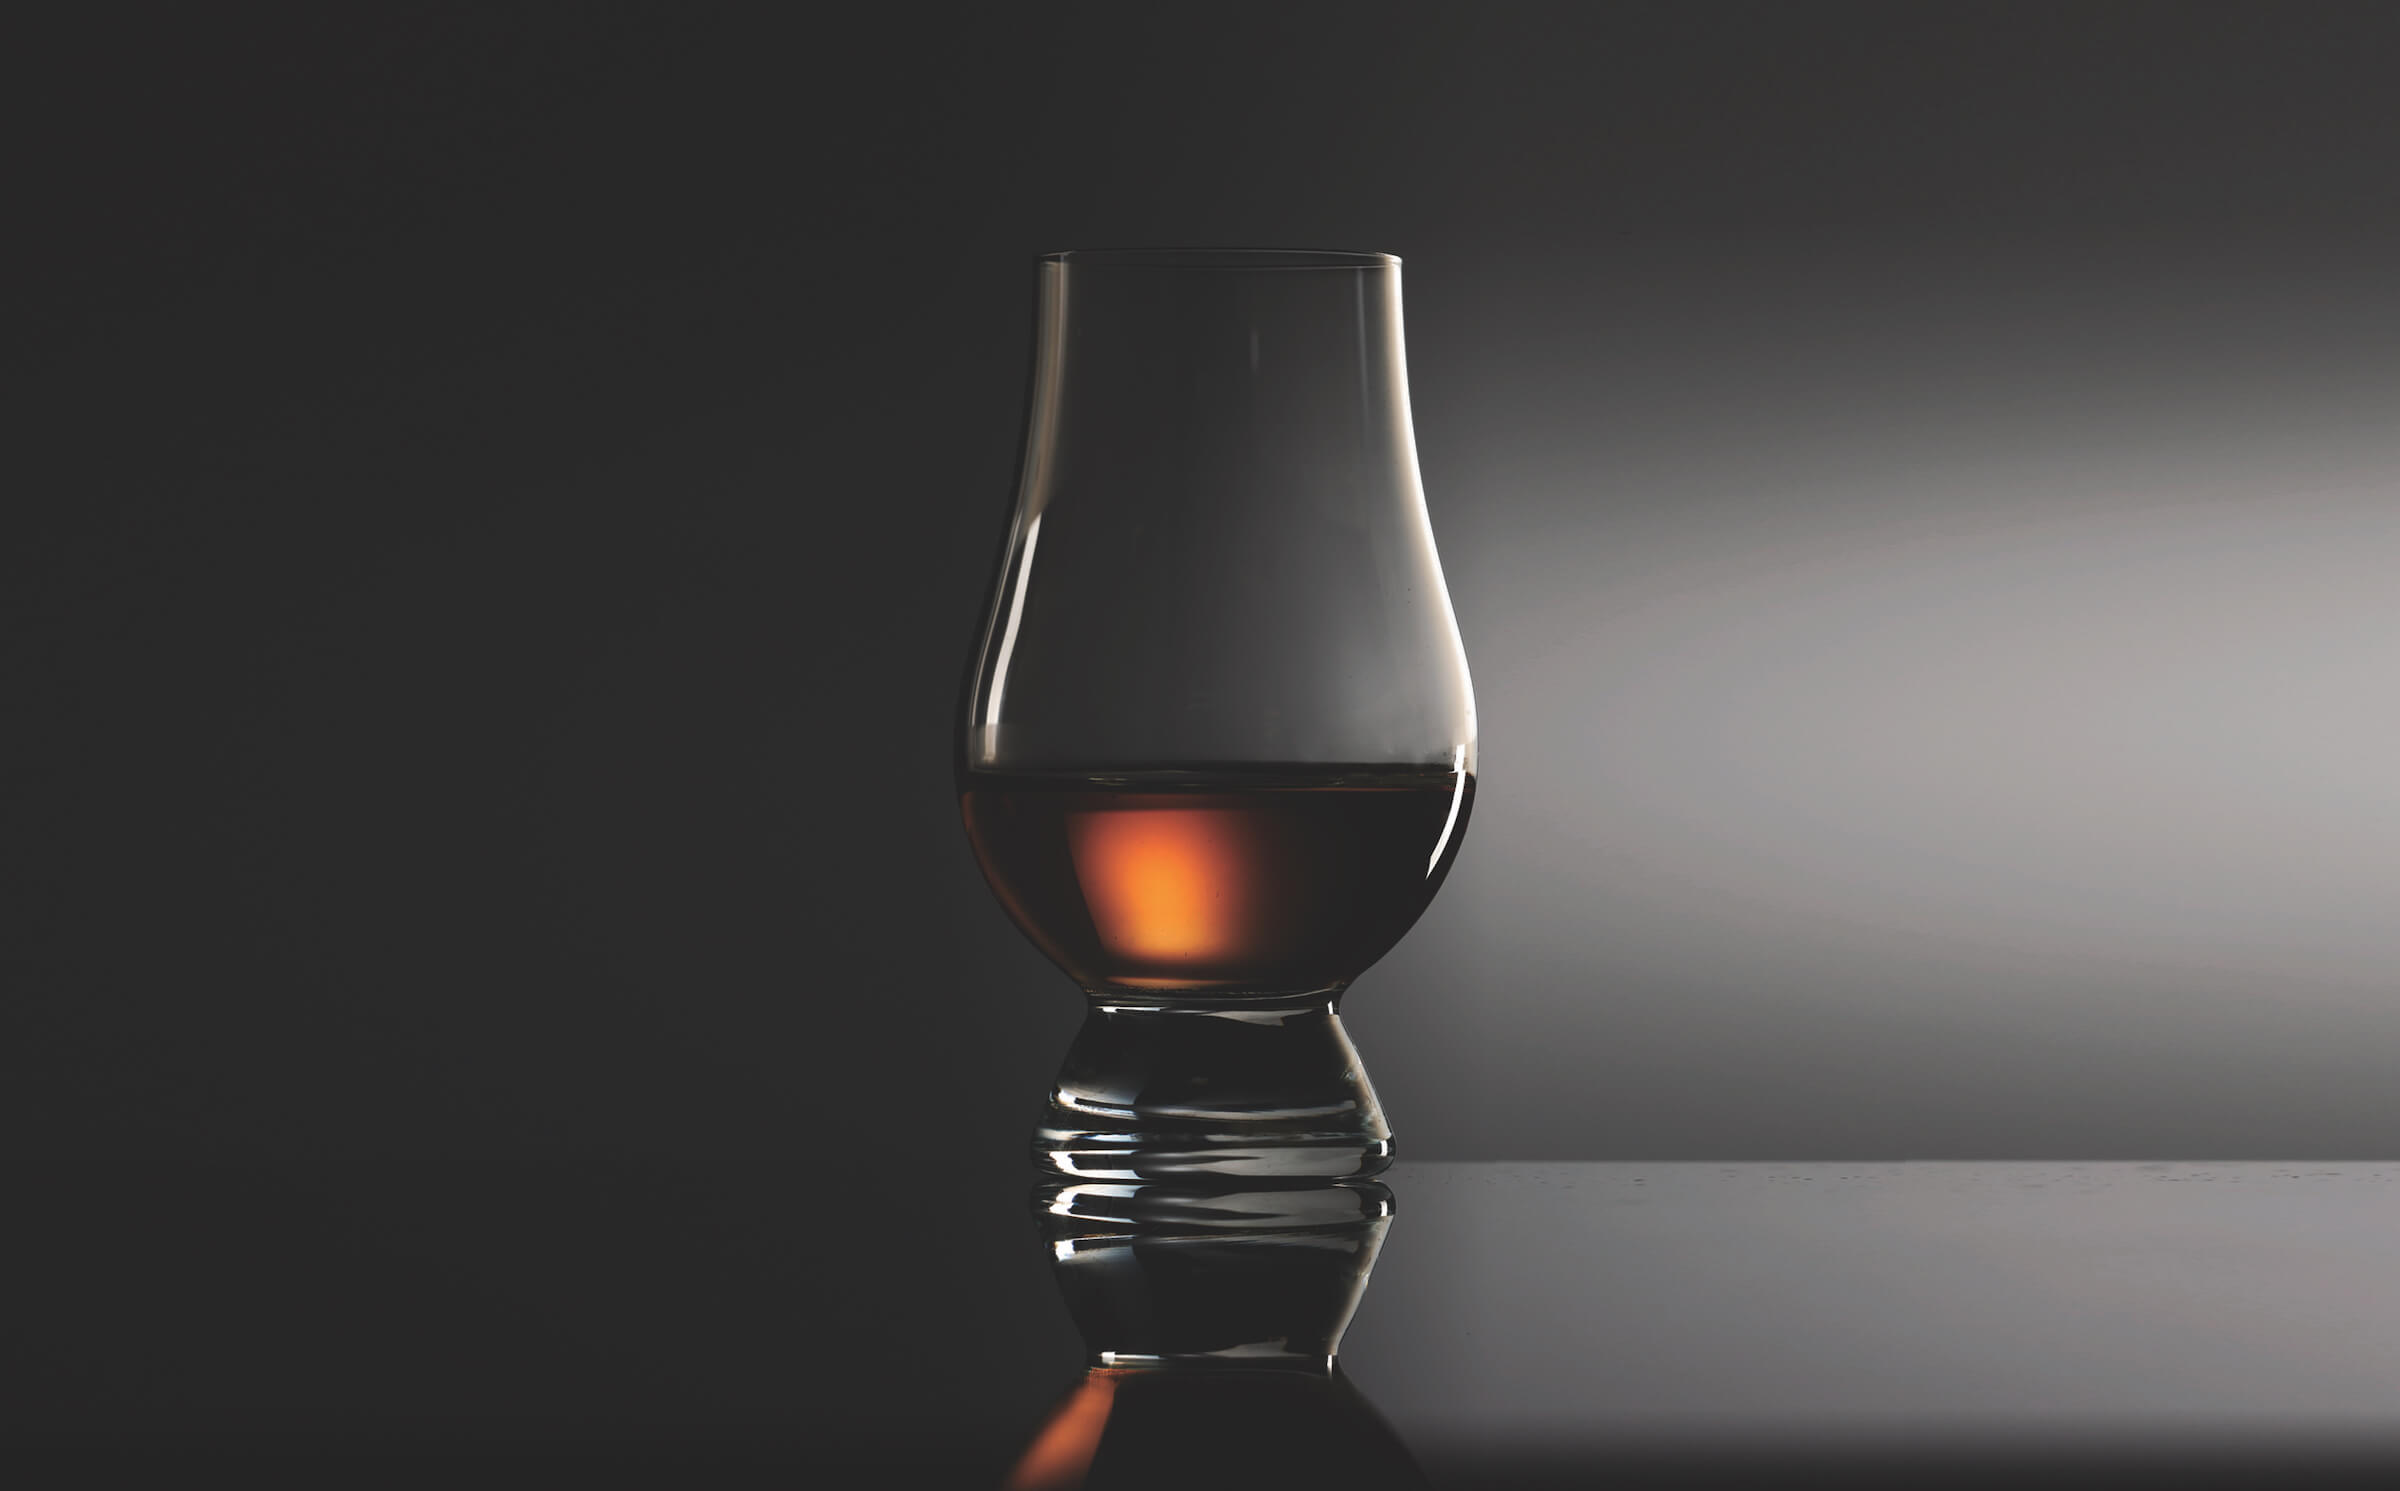
\includegraphics[scale = 0.1]{gwlncairn}
				\end{center}
			
			\end{figure}
	Sugars from dried malted barley fermented, distilled, and aged for years in a numerous possible array of casks. Must be made in Scotland.


	\end{frame}
	\begin{frame}{A complex and long process}
	\begin{columns}
		\begin{column}{0.4\textwidth}
			\begin{figure}[H]
				\begin{center}
					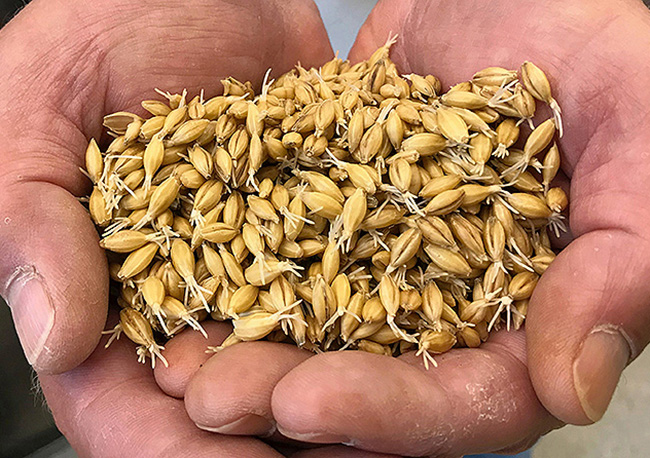
\includegraphics[scale = 0.15]{germ_barley}
					
				\end{center}
			
			\end{figure}
		\end{column}
	
	
		\begin{column}{0.6\textwidth}
			\begin{figure}[H]
				\begin{center}
					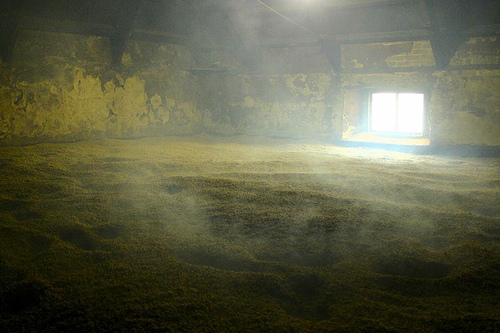
\includegraphics[scale = 0.70]{smoke-dry-barley}
				\end{center}
			\end{figure}
			\begin{figure}[H]
				\begin{center}
					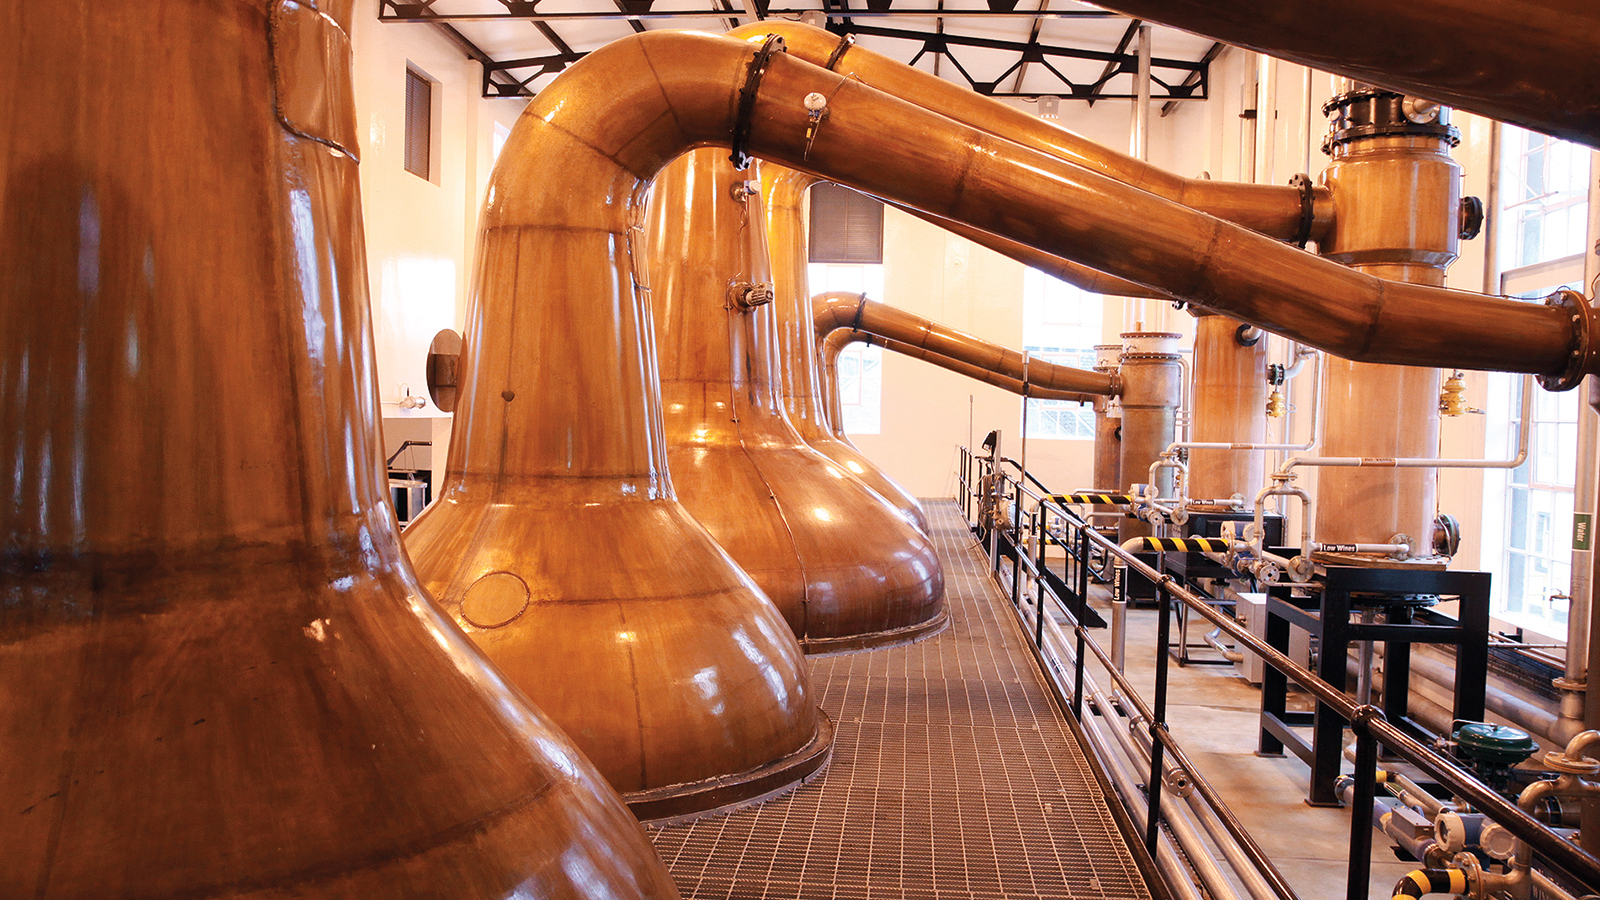
\includegraphics[scale = 0.3]{scotch_stills}
				\end{center}
			\end{figure}
					\begin{figure}[H]
			\begin{center}
				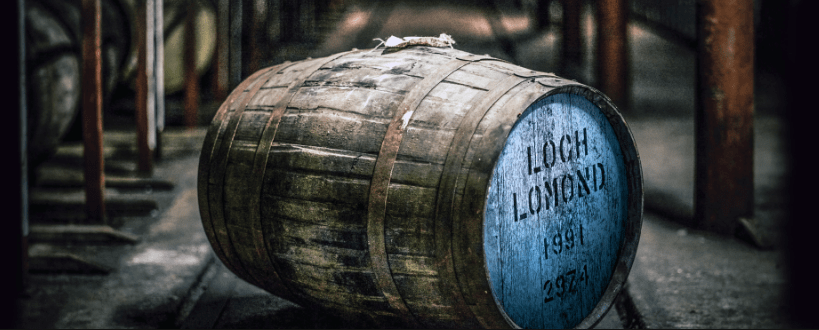
\includegraphics[scale = 0.15]{cask_aging}
			\end{center}
		\end{figure}
	

		\end{column}
		
		
	\end{columns}


\end{frame}
	\begin{frame}{Complex Taste. Colorful lexicon.}
	\begin{columns}
		\begin{column}{0.5\textwidth}
			\begin{itemize}
				\item "The finish dries and becomes pleasantly rubbery, as a touch of truffle oil emerges."
				\item "Seaweed-led, with a hint of vanilla ice cream and more than a whiff of notes from the first aid box (TCP, plasters etc)."
			\end{itemize}

		\end{column}
		\begin{column}{0.5\textwidth}
			\begin{figure}[H]
				\begin{center}
					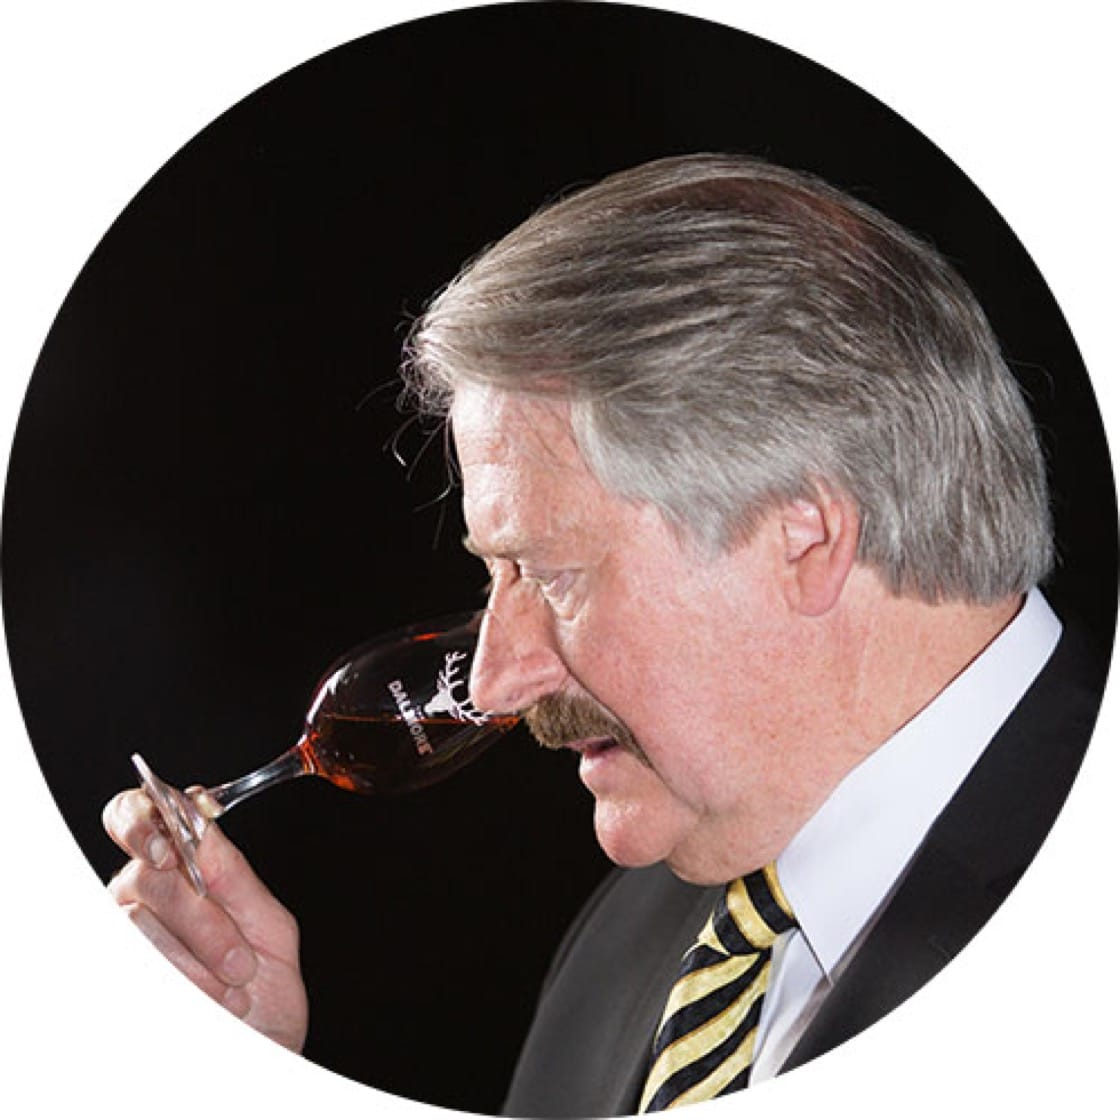
\includegraphics[scale = 0.14]{richpaterson_nosing}
				\end{center}
			\end{figure}
		\end{column}
		
		
	\end{columns}
\end{frame}



\begin{frame}{Making sense of the language}
	\begin{itemize}
		\item Language of Scotch tastes/smells: metaphor, simile
		\item Across a set of Scotch tasting notes:
		\begin{itemize}
			\item Construct lexicon used to describe whisky tastes/smells.
			\item Are there groups of descriptors sharing common themes? Salty, fruity, bittersweet, etc.
			\item Can scotches be described in a more robust way using these groups?
		\end{itemize}
	\end{itemize}
\end{frame}





	\begin{frame}{Getting expert tasting notes}


	\begin{columns}
		\begin{column}{0.4\textwidth}
		\begin{figure}
			
			
\includegraphics[scale = 0.2]{masterofmalt}
			
		\end{figure}
		\end{column}
		\begin{column}{0.6\textwidth}

		Master of Malt (MoM): online store + expert tasting notes from The Chaps at MoM.


		\end{column}
		
	\end{columns}
	Scrapy spider: extract tasting notes + bottling details on $\approx$ 8,600 Scotches
\end{frame}

	\begin{frame}{Getting expert tasting notes}
	
	

			\begin{figure}
				
				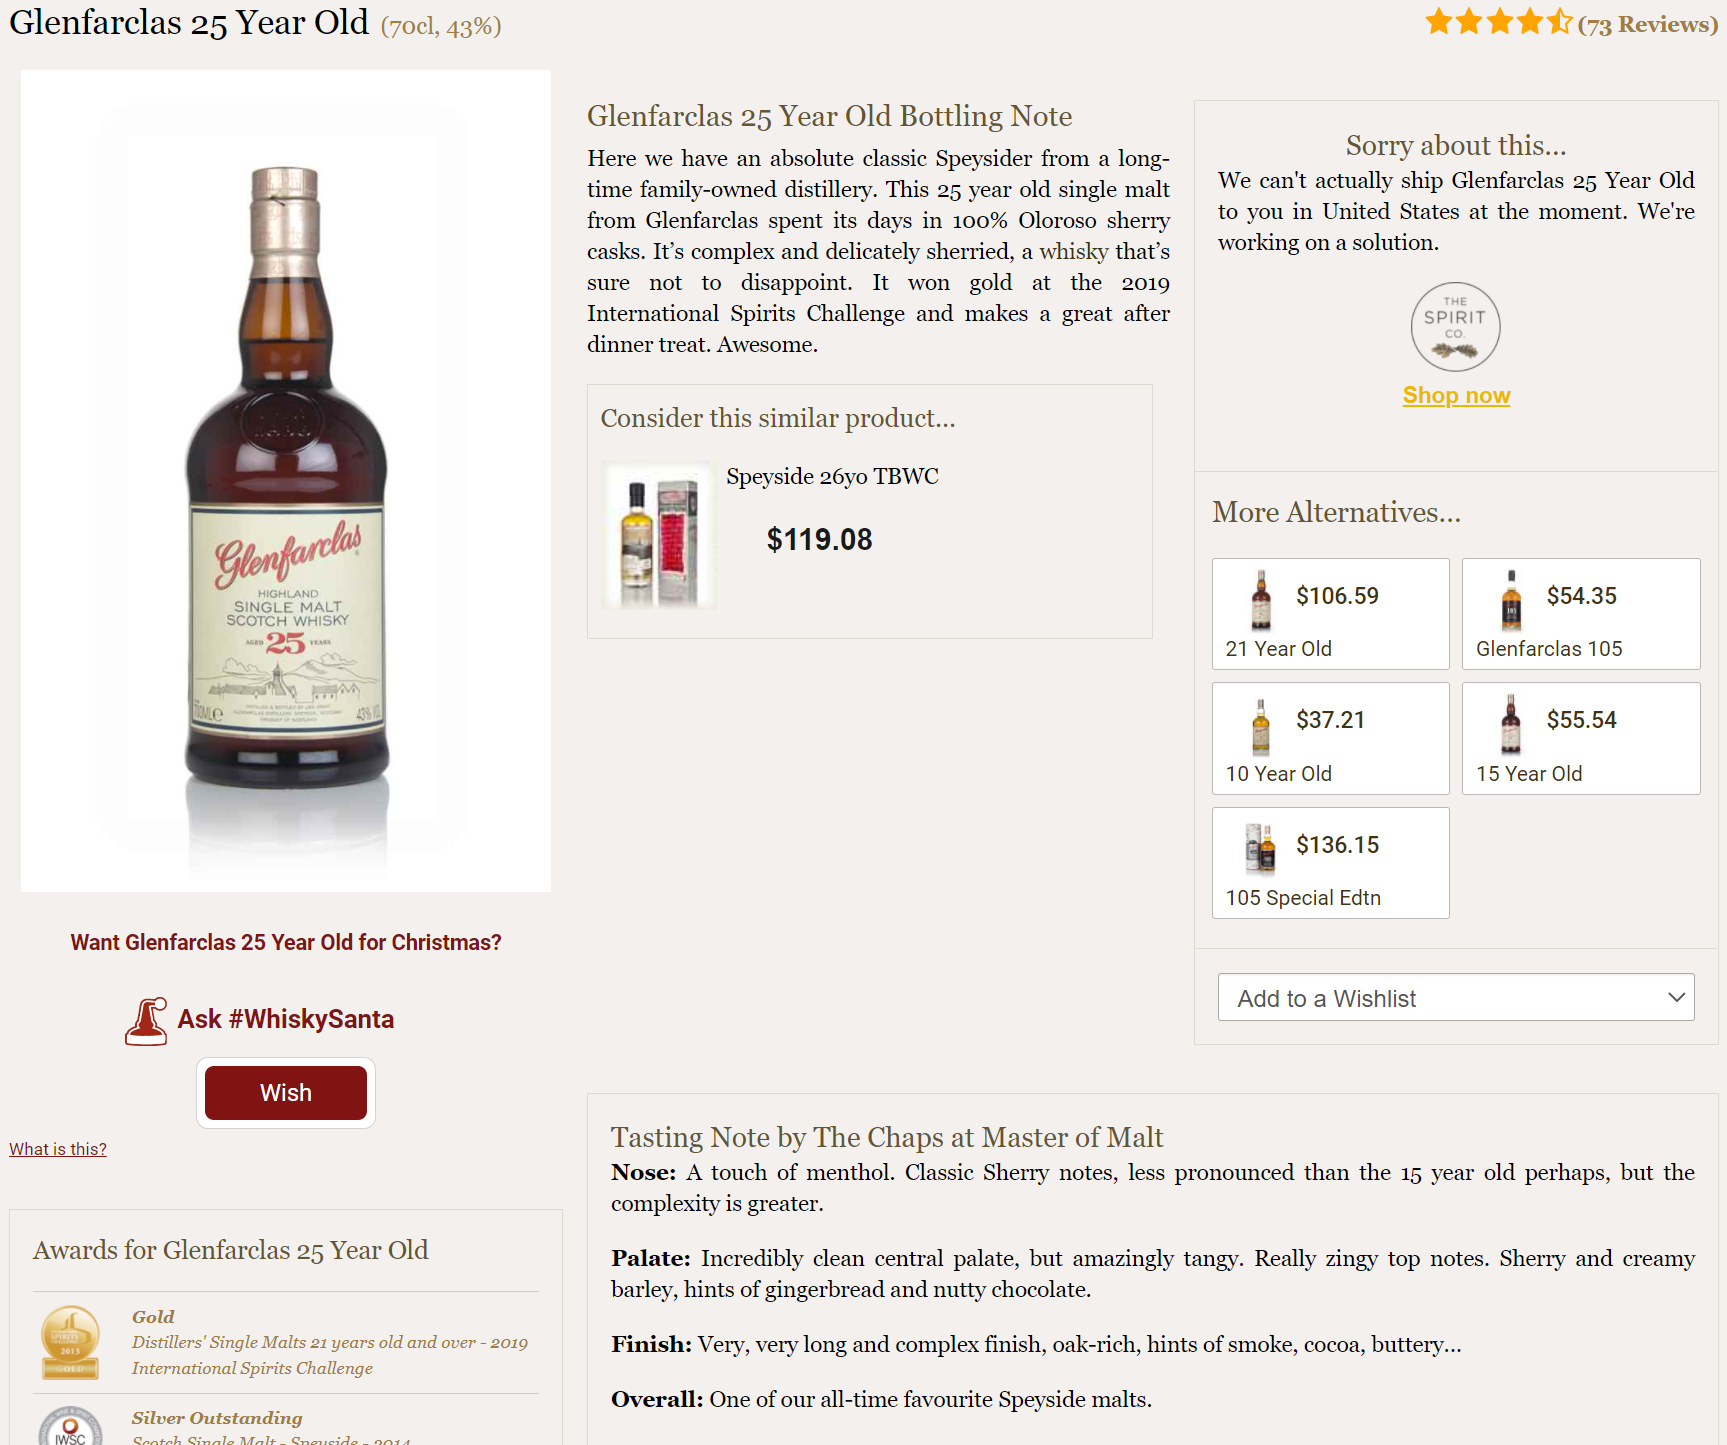
\includegraphics[scale = 0.4]{product_page}
				
			\end{figure}

\end{frame}

	\begin{frame}{Extracted Information}
	
	\begin{table}[H]
		\begin{center}
		\begin{tabular}{|c|c|}
			\hline
			name &  The name of the scotch.\\
			\hline
			distillery &  Distillery that produced the scotch.\\
			\hline
			bottler &  Some scotches are aged/bottled by 3rd parties. \\
			\hline
			region & Whisky making region that the distillery belongs to. \\
			\hline
			age & Maturation time (in years).  \\
			\hline
			ABV & Alcohol by volume. \\
			\hline
			price & MoM is also a store. Price in USD.  \\
			\hline
			description & General notes about the Scotch.  \\
			\hline
			nose & Free text description of the scent of the Scotch.  \\
			\hline
			palate & Free text description of the taste of the whisky. \\
			\hline
			finish & Free text description of aftertastes.  \\
			\hline
			chill filter & Is the whisky chill filtered? \\
			\hline
			cask strength & Is the whisky bottled at cask strength? \\
			\hline
			maturation & Cask(s) used to age the whisky. \\
			
			\hline
		\end{tabular}
		\caption{Scotch attributes scraped from MoM.}
	\end{center}
	\end{table}
	
	
\end{frame}

\begin{frame}{Text Preprocessing/Normalization}
\begin{columns}
	\begin{column}{0.6\textwidth}
		\begin{figure}[H]
			\begin{center}
				
\includegraphics[scale = 0.08]{spacy}
			\end{center}
		\end{figure}
	\end{column}
\begin{column}{0.6\textwidth}
	\begin{figure}[H]
		\begin{center}
			
\includegraphics[scale = 0.3]{gensim}
		\end{center}
	\end{figure}
\end{column}
\end{columns}
\begin{block}{Text Processing Flow}
	
	\begin{adjustbox}{max totalsize={.9\textwidth}{.7\textheight},center}
		
		\begin{tikzpicture}[auto]
			
			\node [block] (start) {nose};
			\node [block, below = 1 cm of start] (start2) {palate};
			\node [block, below = 1 cm of start2] (start3) {finish};
			\node [block, right =1cm of start2] (unified) {Unified text};
			
			\node[block, right =1cm of unified] (spacy) {spaCy pipeline:\\ tokenizer, lemmatizer, token removal};		
			
			\node[block, right =1cm of spacy] (phraser) {Gensim Phrase model: probable Bigrams};
			
			\node[block, right =1cm of phraser] (manualstem) {Manual stemming: Regex};
			
			

			
			
			
			%% paths
			\path[draw,->]
			(start2) edge (unified)
			(unified) edge (spacy)
			(spacy) edge (phraser)
			(phraser) edge (manualstem)
			;
			
			\path [line] (start) -| (unified);
			\path [line] (start3) -| (unified);
		\end{tikzpicture}
		
	\end{adjustbox}
	
\end{block}
\end{frame}

\begin{frame}{Dictionary and corpus generation}
\begin{columns}
\begin{column}{0.5\textwidth}
\begin{itemize}
	\item Gensim dictionary from tokens
		\begin{itemize}
		\item 4145 unique descriptors
	\end{itemize}
	\item Filter tokens: 
	\begin{itemize}
		\item Lower bound: 0.5\%  of reviews
		\item Upper bound 50\% of reviews
		\item Reduced dictionary: 477 descriptors
	\end{itemize}
	
	\item Bag-of-words (BoW) representation
		\begin{itemize}
		\item Gensim corpus
		\item Sparse review/descriptor-frequency matrix
	\end{itemize}
	
\end{itemize}
\end{column}
\begin{column}{0.5\textwidth}
	\begin{figure}[H]
		\begin{center}
			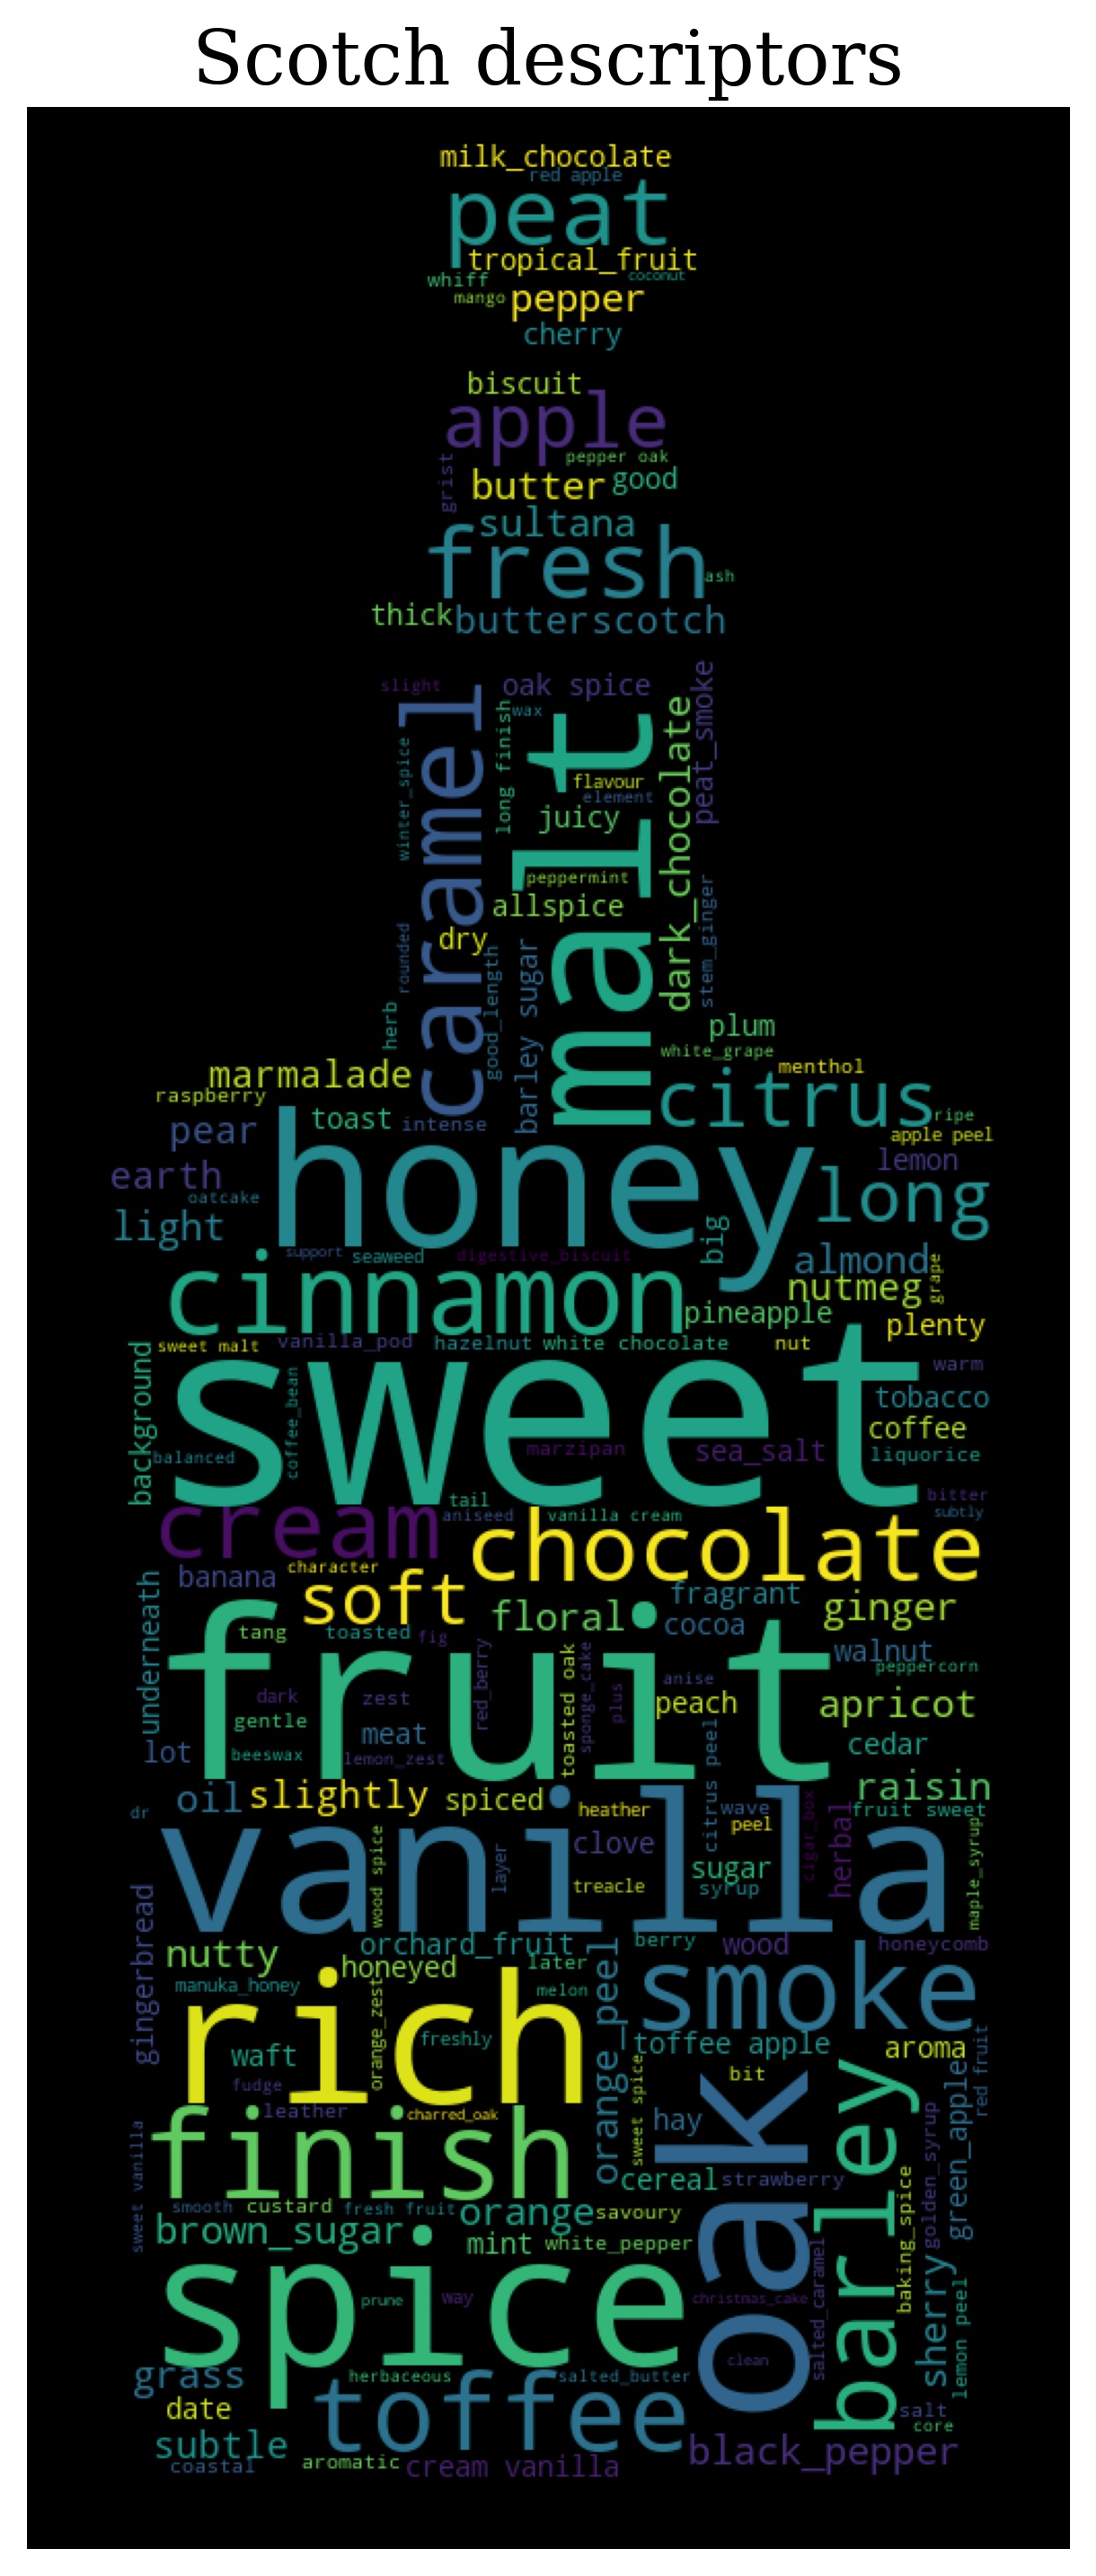
\includegraphics[scale = 0.32]{wc_token_unified}
		\end{center}
	\end{figure}
\end{column}
\end{columns}
\end{frame}
\begin{frame}{Descriptors}
	\begin{columns}
		\begin{column}{0.5\textwidth}
			\begin{itemize}
				\item Common descriptors: sweet, vanilla, fruit, spice, oak, malt, etc.
				\item Groupings among descriptors: taste types?
				\item Regional differences

				
			\end{itemize}
		\end{column}
		\begin{column}{0.5\textwidth}
			\begin{figure}[H]
				\begin{center}
					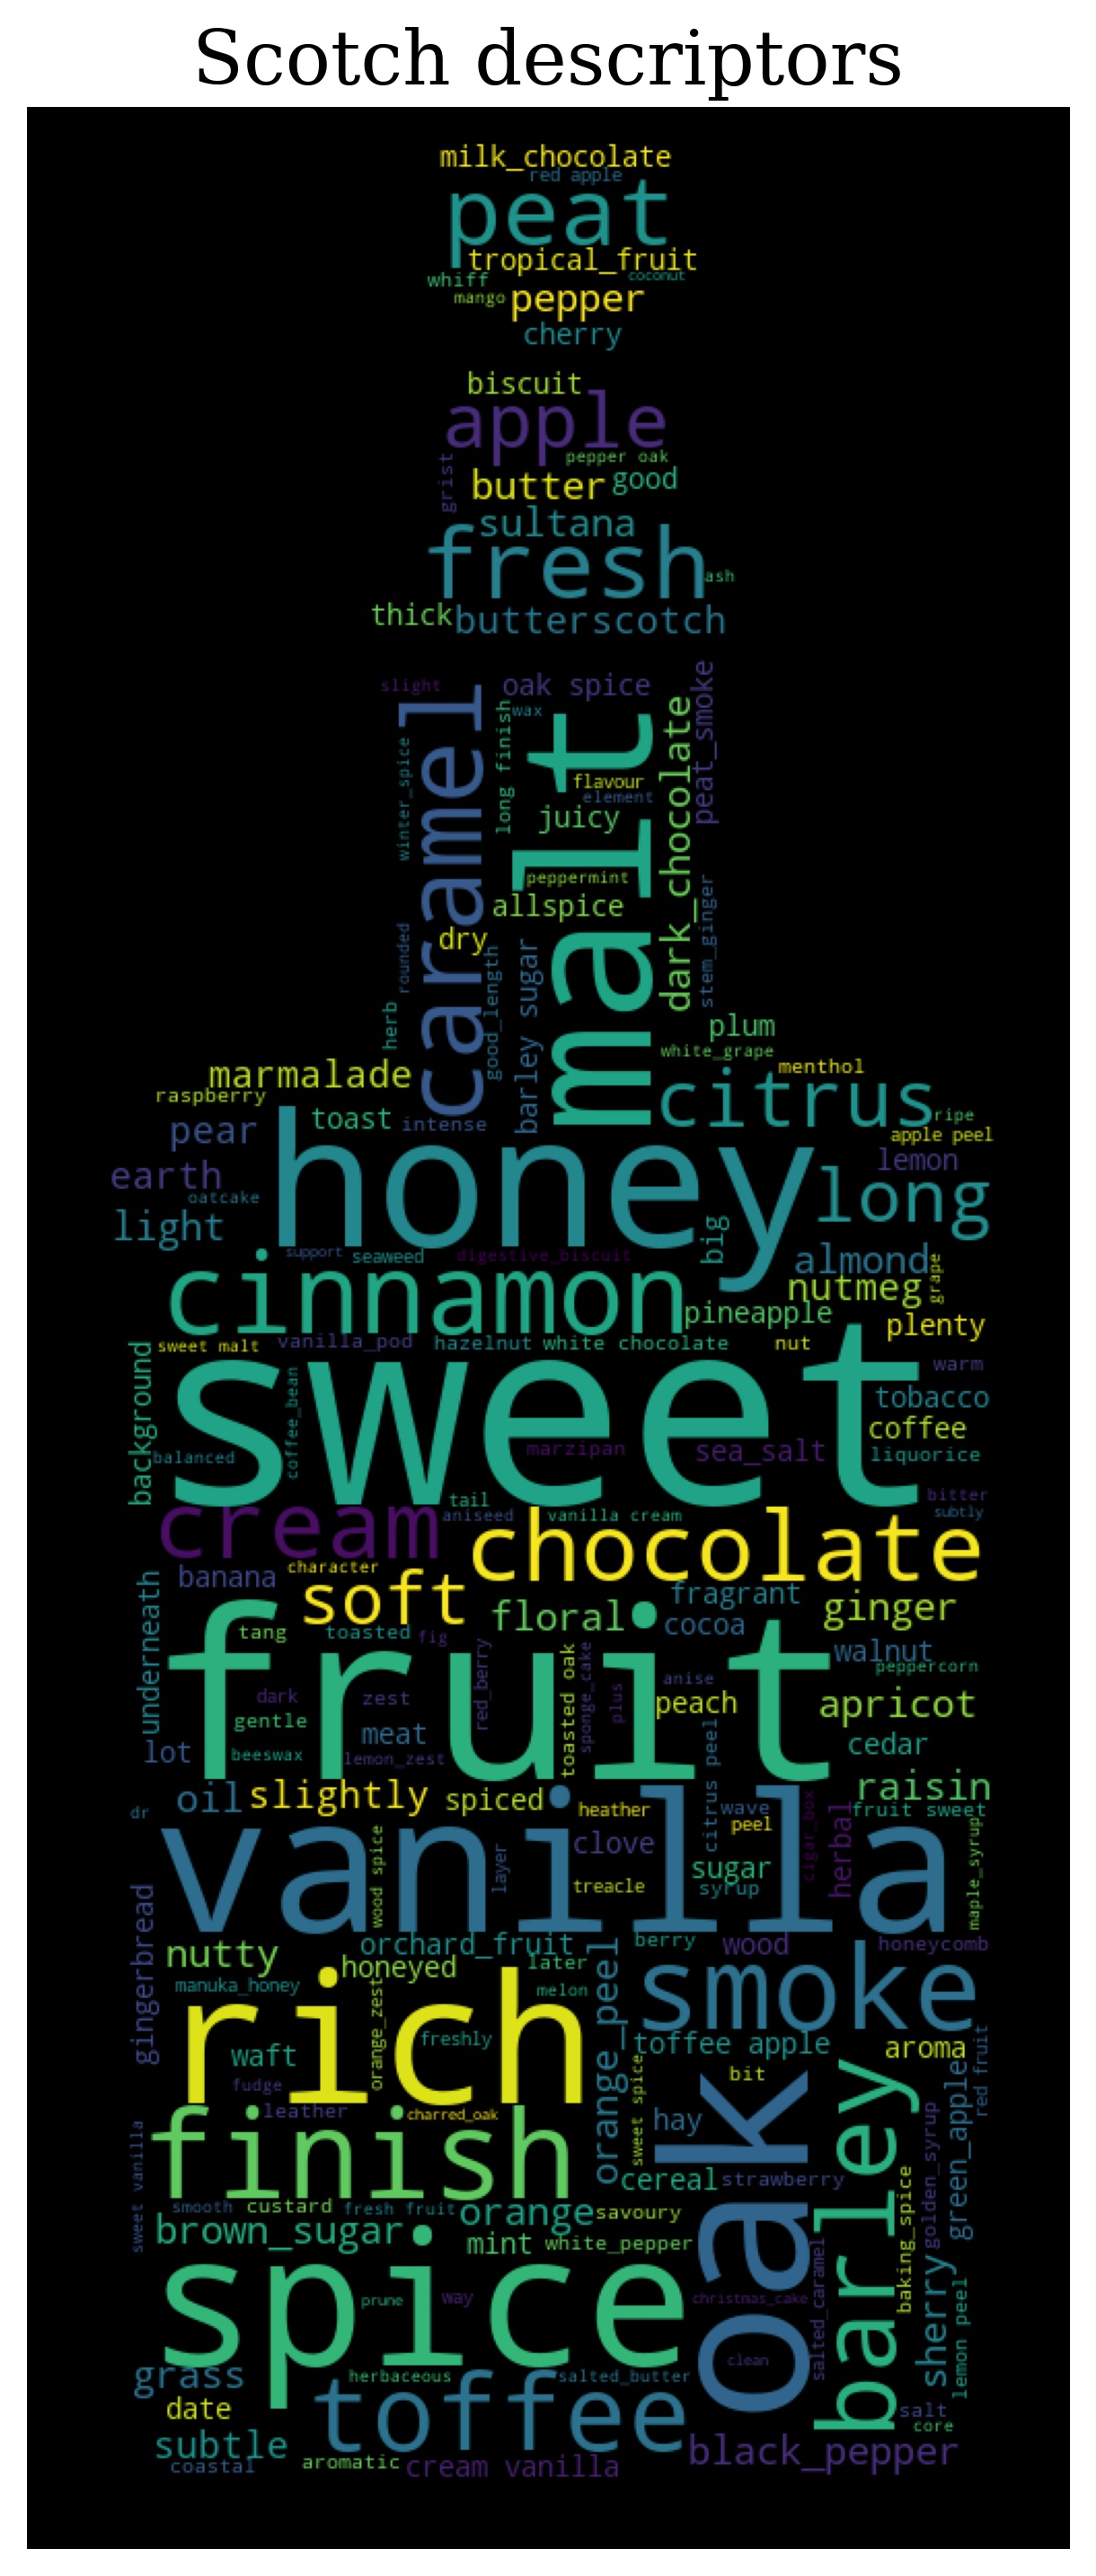
\includegraphics[scale = 0.32]{wc_token_unified}
				\end{center}
			\end{figure}
		\end{column}
	\end{columns}
\end{frame}

\begin{frame}{Scotch producing regions}
	\begin{columns}
		\begin{column}{0.5\textwidth}
			Scotches from different regions are said to have certain character. Let's see.
		\end{column}
	\begin{column}{0.5\textwidth}
	\begin{figure}[H]
		\begin{center}
			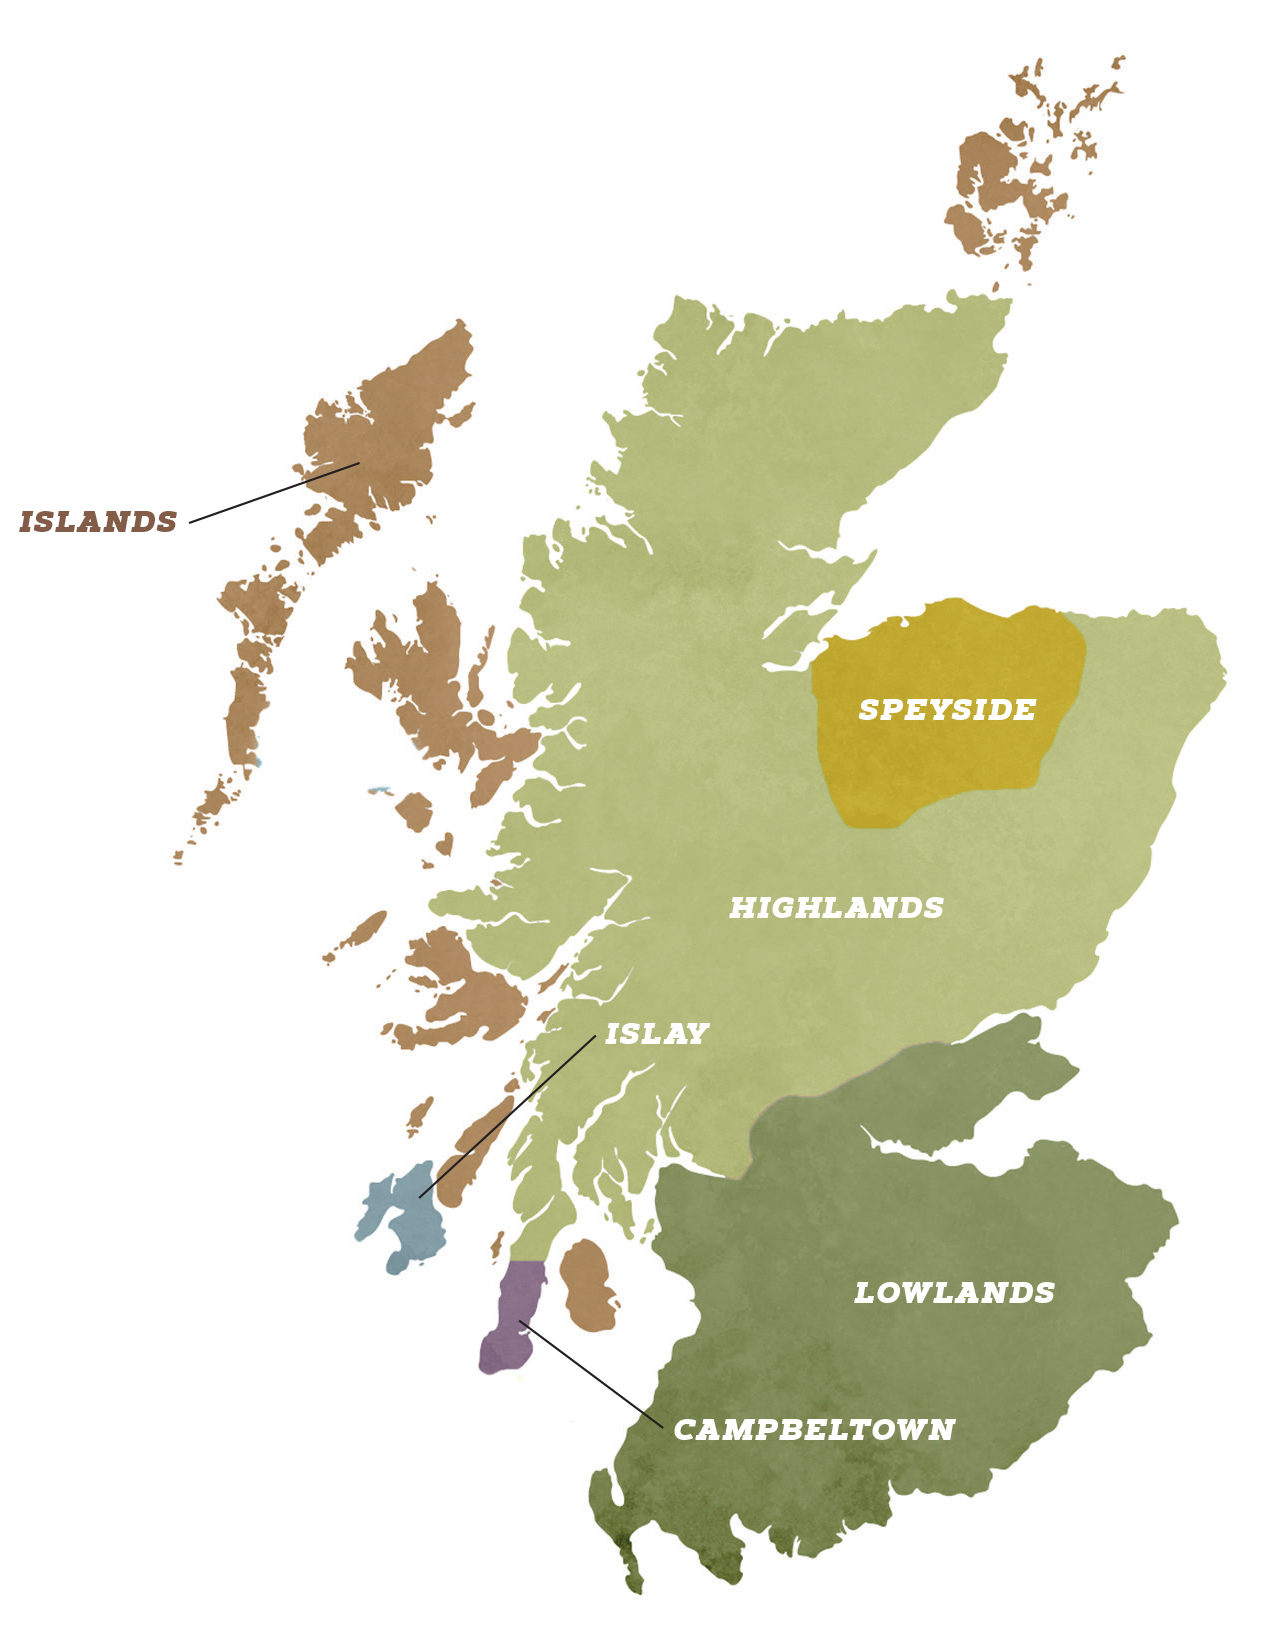
\includegraphics[scale = 0.55]{scotland_regions}
		\end{center}
	\end{figure}
\end{column}

\end{columns}
\end{frame}

\begin{frame}{Correspondence Analysis (CA)}
	Visualize descriptors and their groupings in a low-dimensional space.
	\begin{itemize}
		\item CA embeds descriptors in low-D space: similar co-occurence of descriptors across reviews are related.
		\item  Document/term-frequency correlations: embed tasting notes / scotches in same space as descriptors.
		\item \textit{Technical}:
		\begin{itemize} 
			\item Double-center document/term-frequency matrix. 
			\item Take residual (co-occurences beyond what is expected on average), SVD.
			\item Project into 2D (first two singular values). Symmetrize bases for descriptors and scotches for 2D embedding.
			\end{itemize}
	\end{itemize}
\end{frame}
	\begin{frame}{Correspondence Analysis: Descriptors}
	\begin{figure}[H]
		\begin{center}
			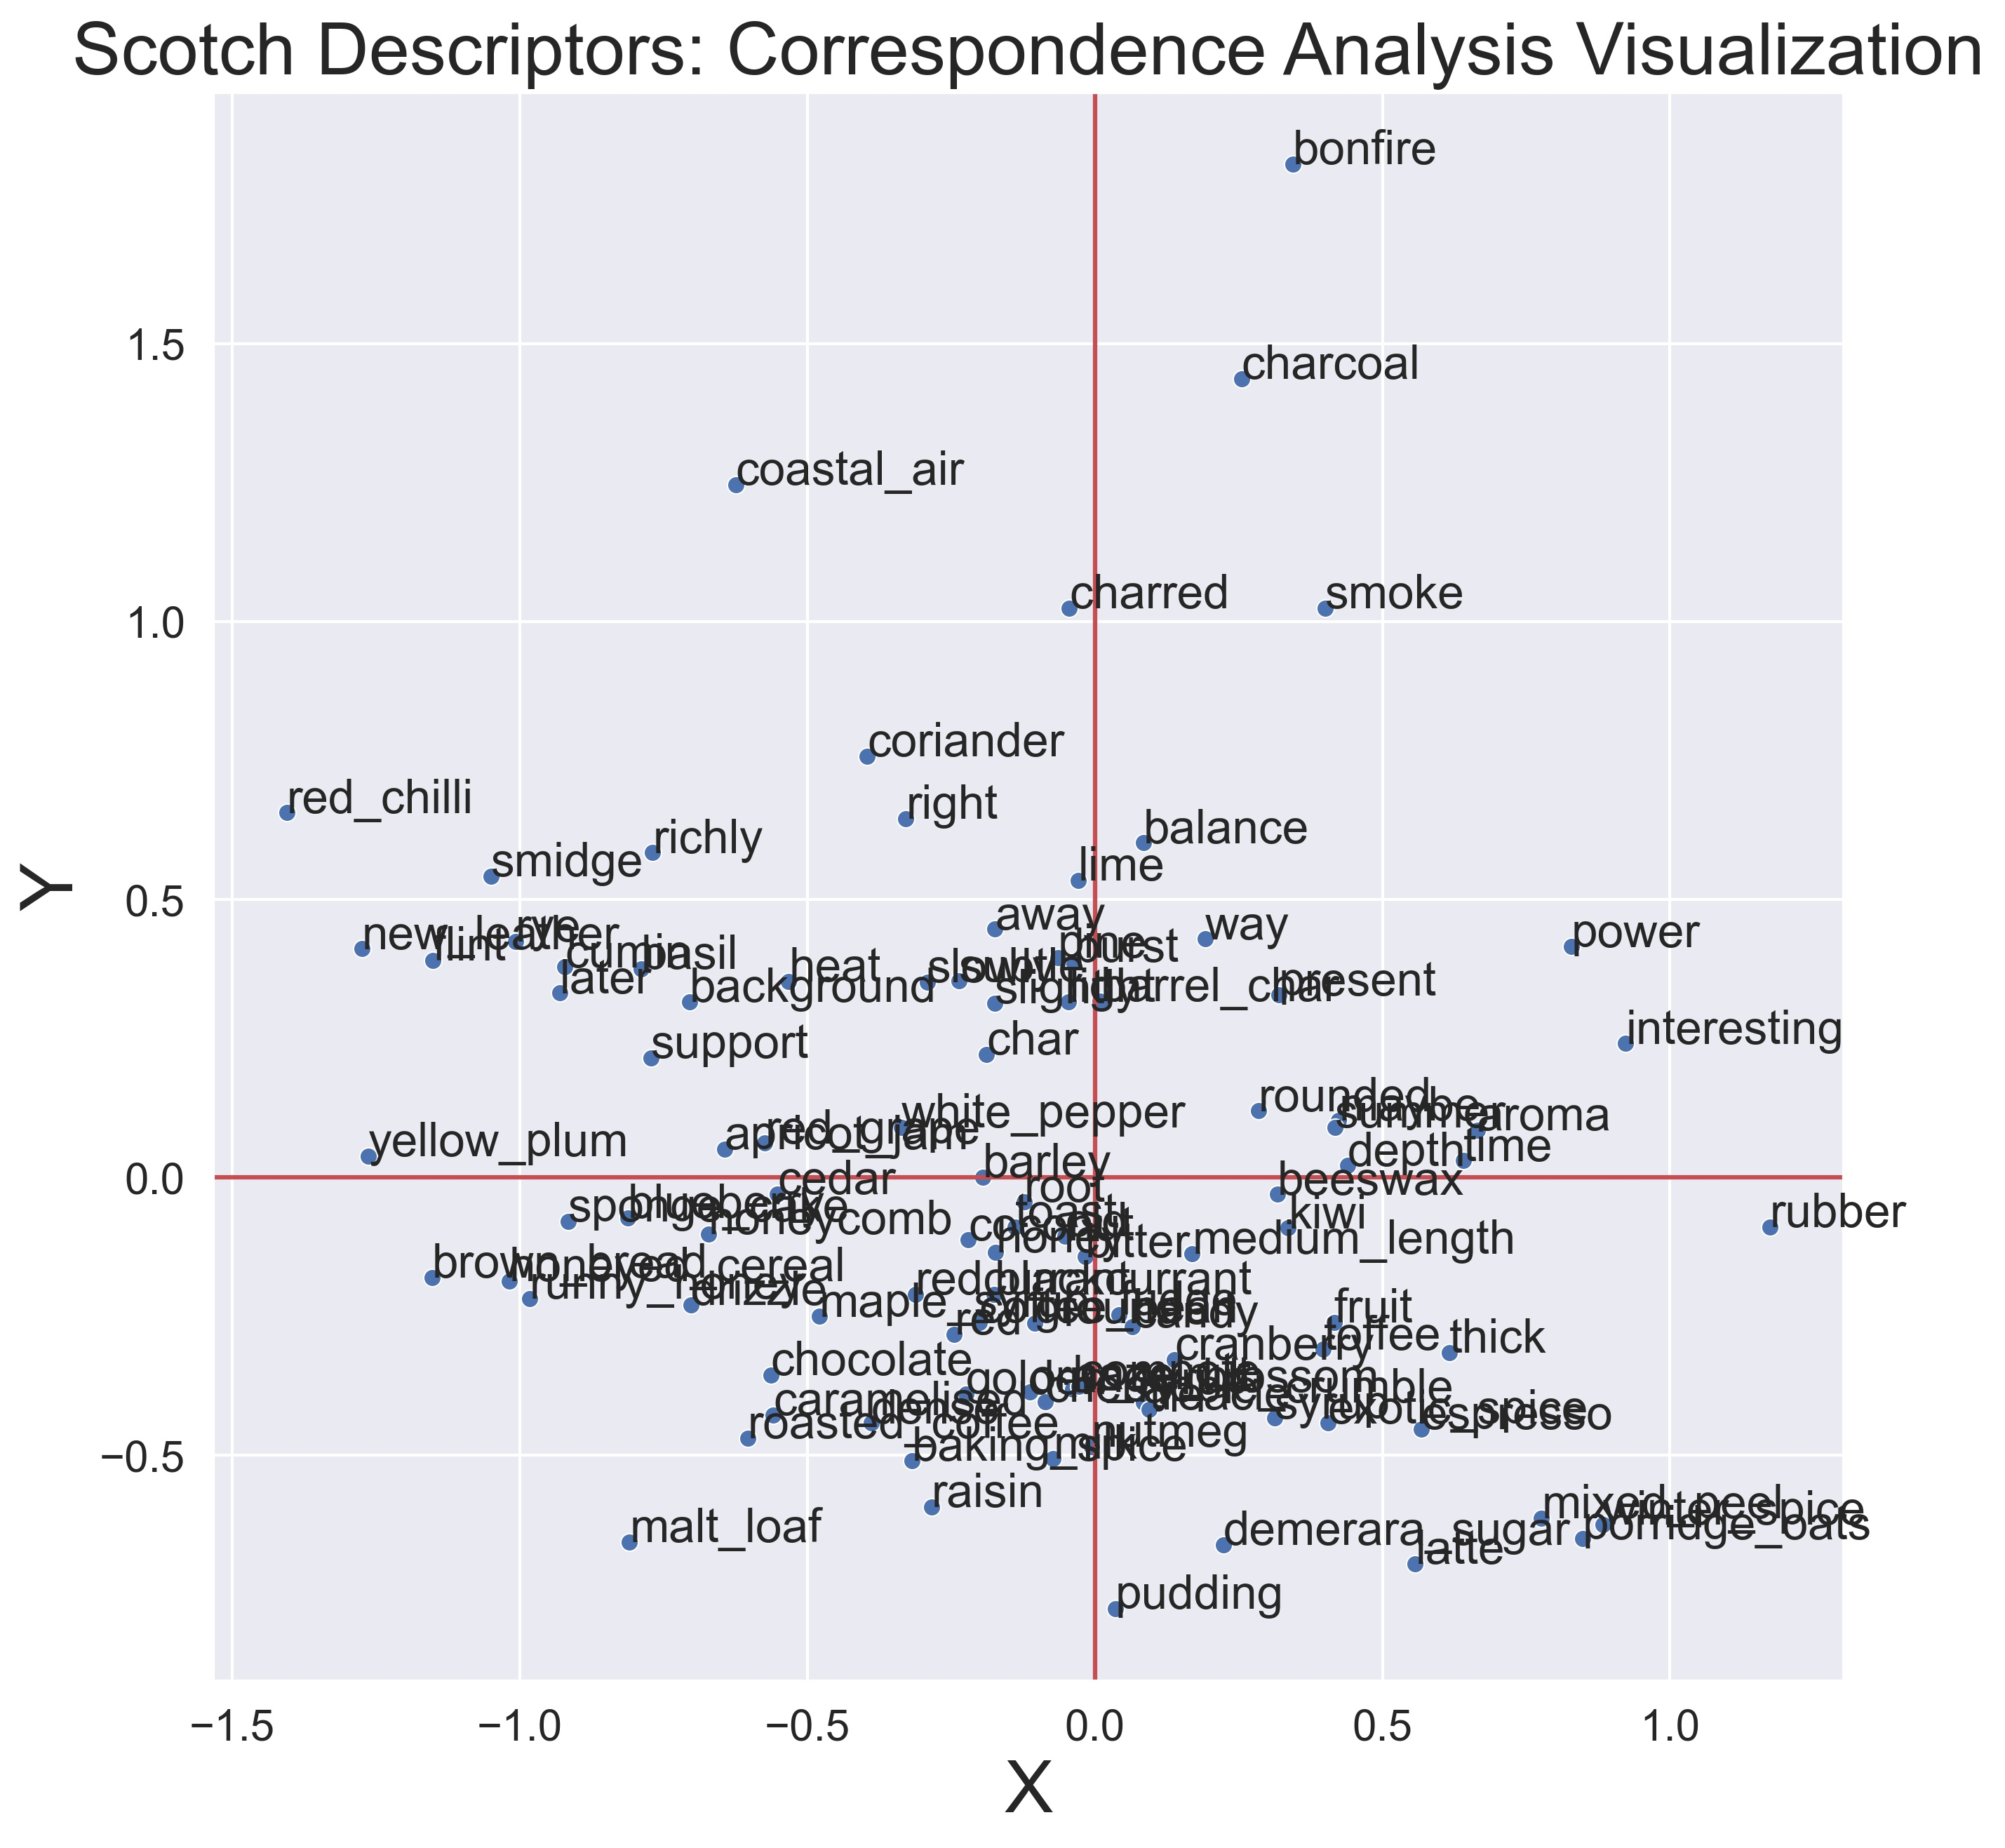
\includegraphics[scale = 0.35]{cawordembed}
		\end{center}
	\end{figure}
\end{frame}
	\begin{frame}{Correspondence Analysis: Scotches by region}
		\begin{figure}[H]
		\begin{center}
			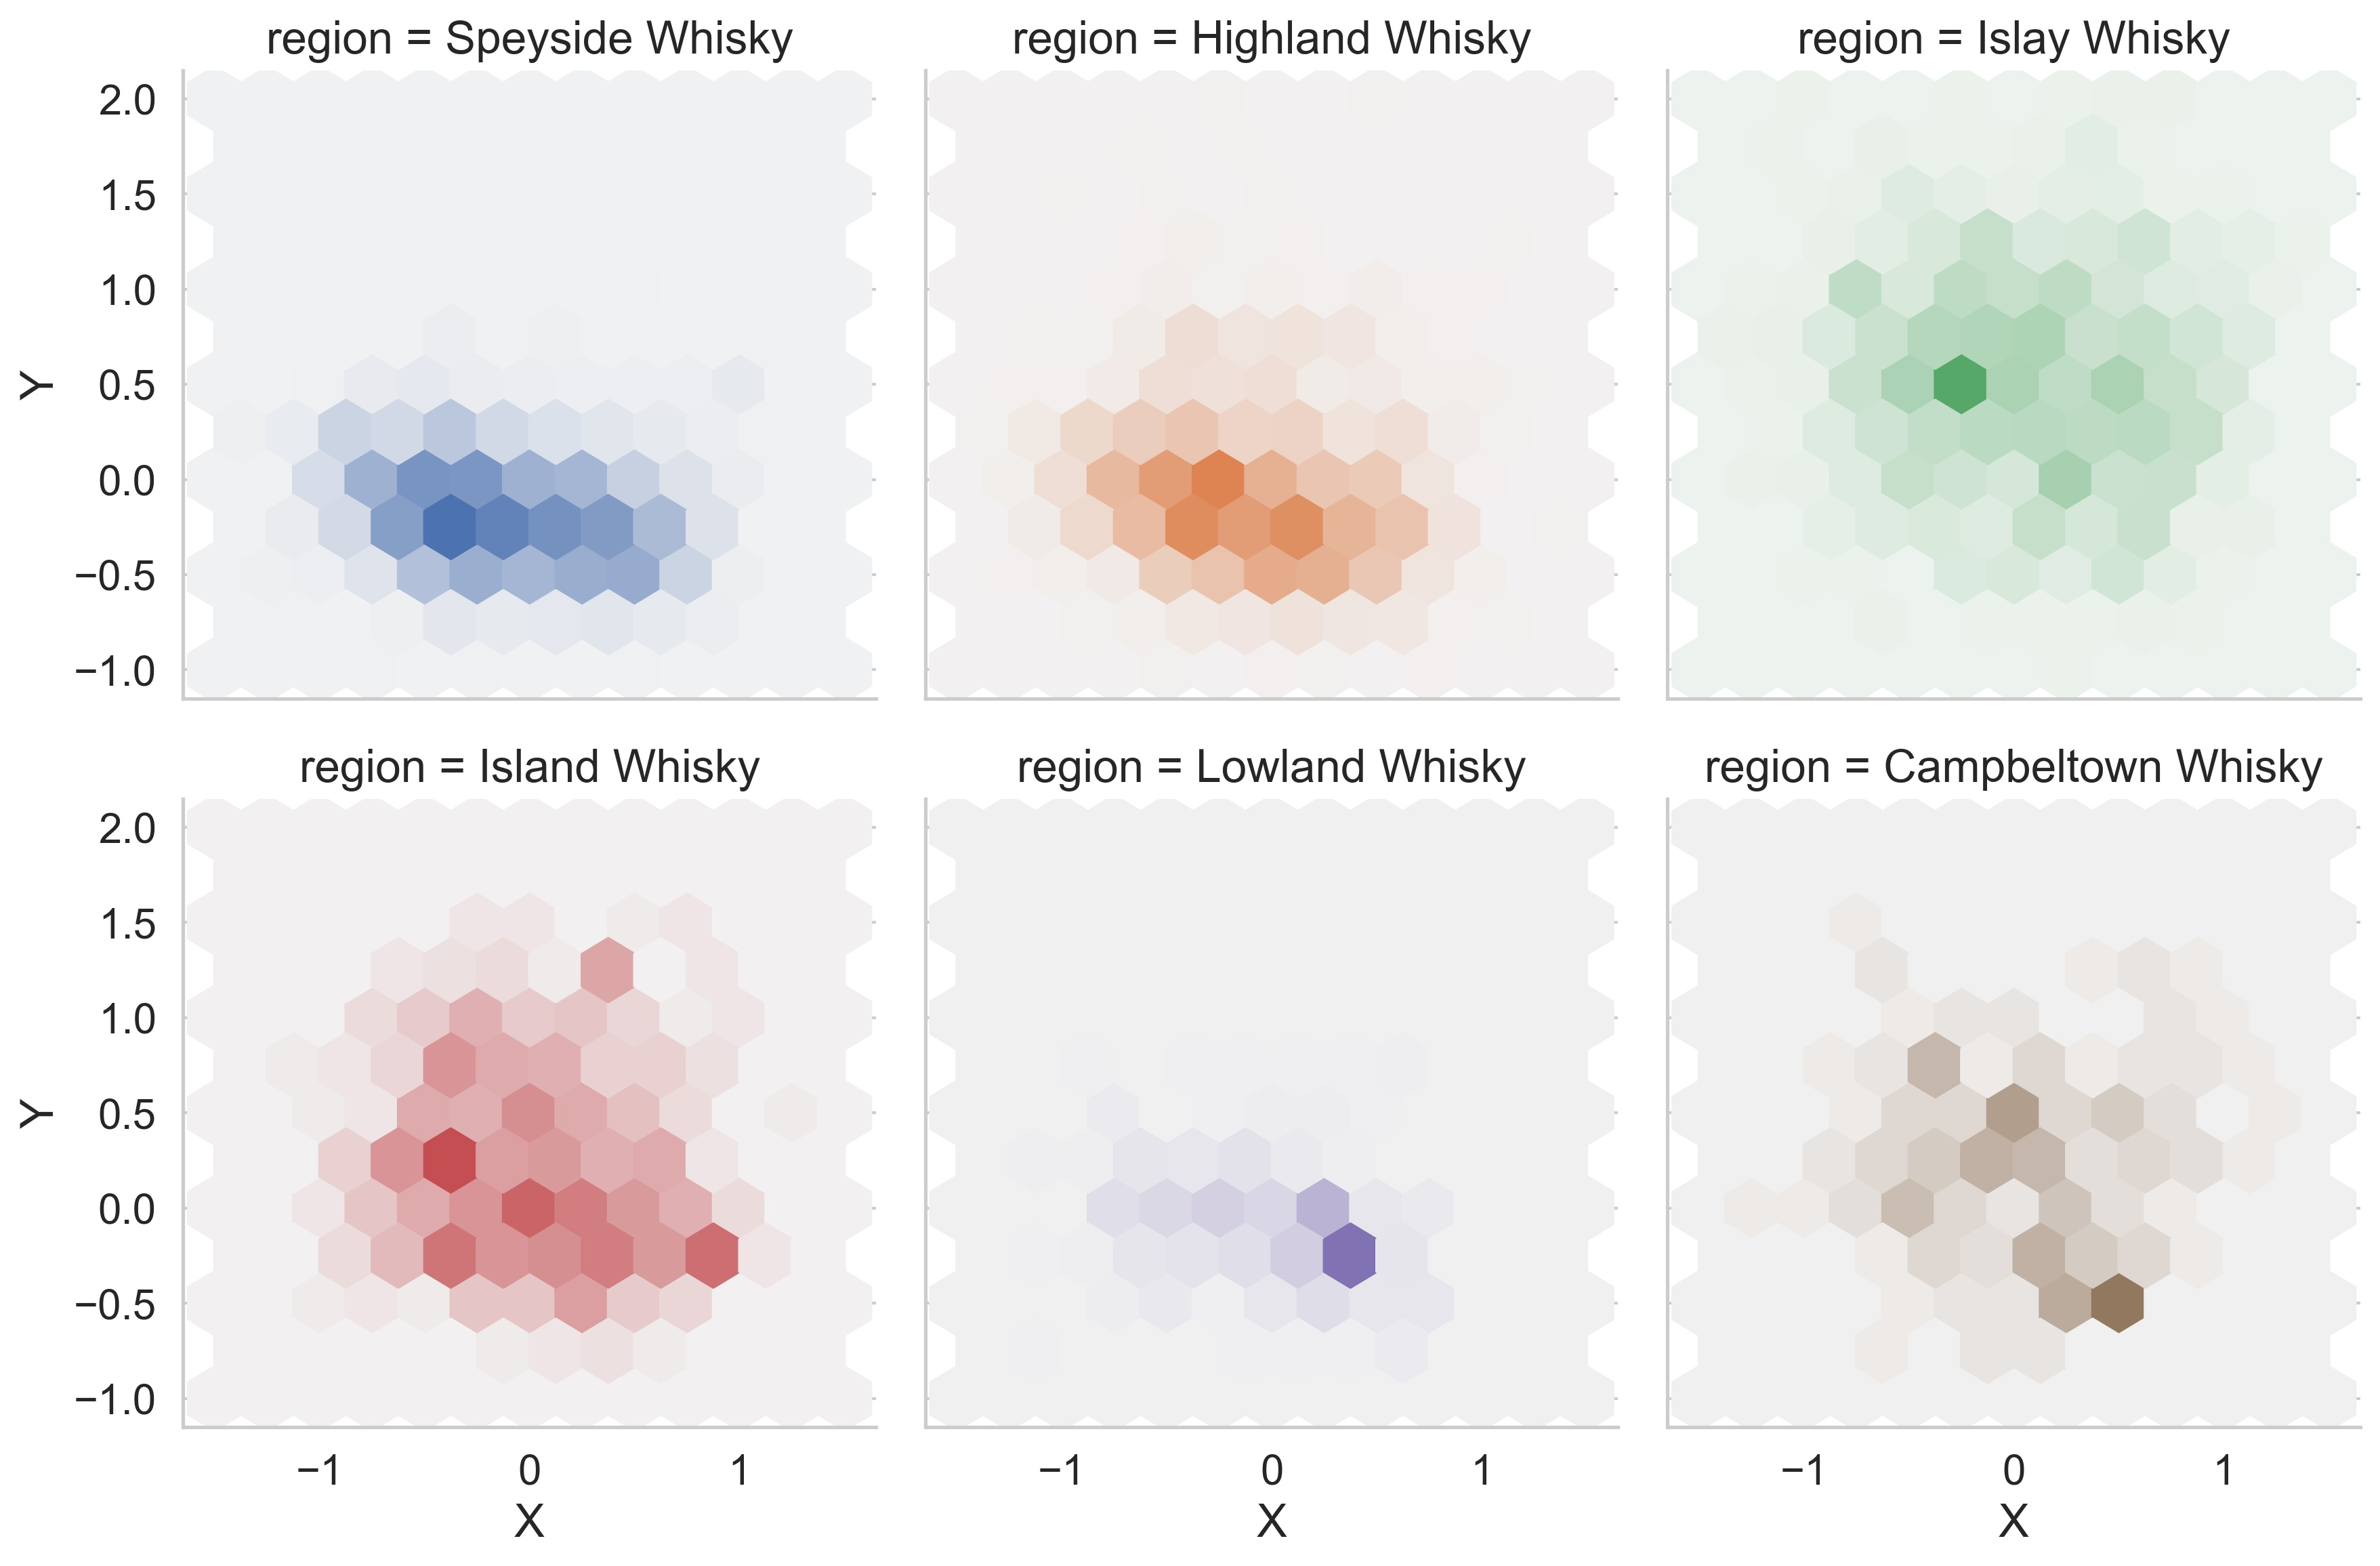
\includegraphics[scale = 0.35]{CA_scotch_hexdistbyregion}
		\end{center}
	\end{figure}
Scotches likely exhibit multiple flavor types. Flavor breakdown?
\end{frame}
\begin{frame}{Topic Modeling}
	Want to construct groups of descriptors and break each tasting note down into a combination of these groups.
\begin{itemize}	
	\item Latent Dirichlet Allocation (LDA)
	\item Assume $K$ topics (taste groups)
	\item Two-level probabilistic inference: 
	\begin{itemize}
		\item Distribution of topics on each document (tasting note)
		\item Distribution of tokens in each topic
	\end{itemize}
	\item Nice thing about LDA: Human interpretable topics.
\end{itemize}
	
\end{frame}
	\begin{frame}{Tuning the number of topics}
		Number of topics as model hyperparameter. 
	\begin{columns}
		\begin{column}{0.4\textwidth}
\begin{itemize}
	\item Tuning for human interpretability.
	\item Quantitative measures? 
	\item $c_v$ score: agg. mutual info between descriptors in topic
\end{itemize}

		\end{column}
		\begin{column}{0.6\textwidth}
			\begin{figure}[H]
				\begin{center}
					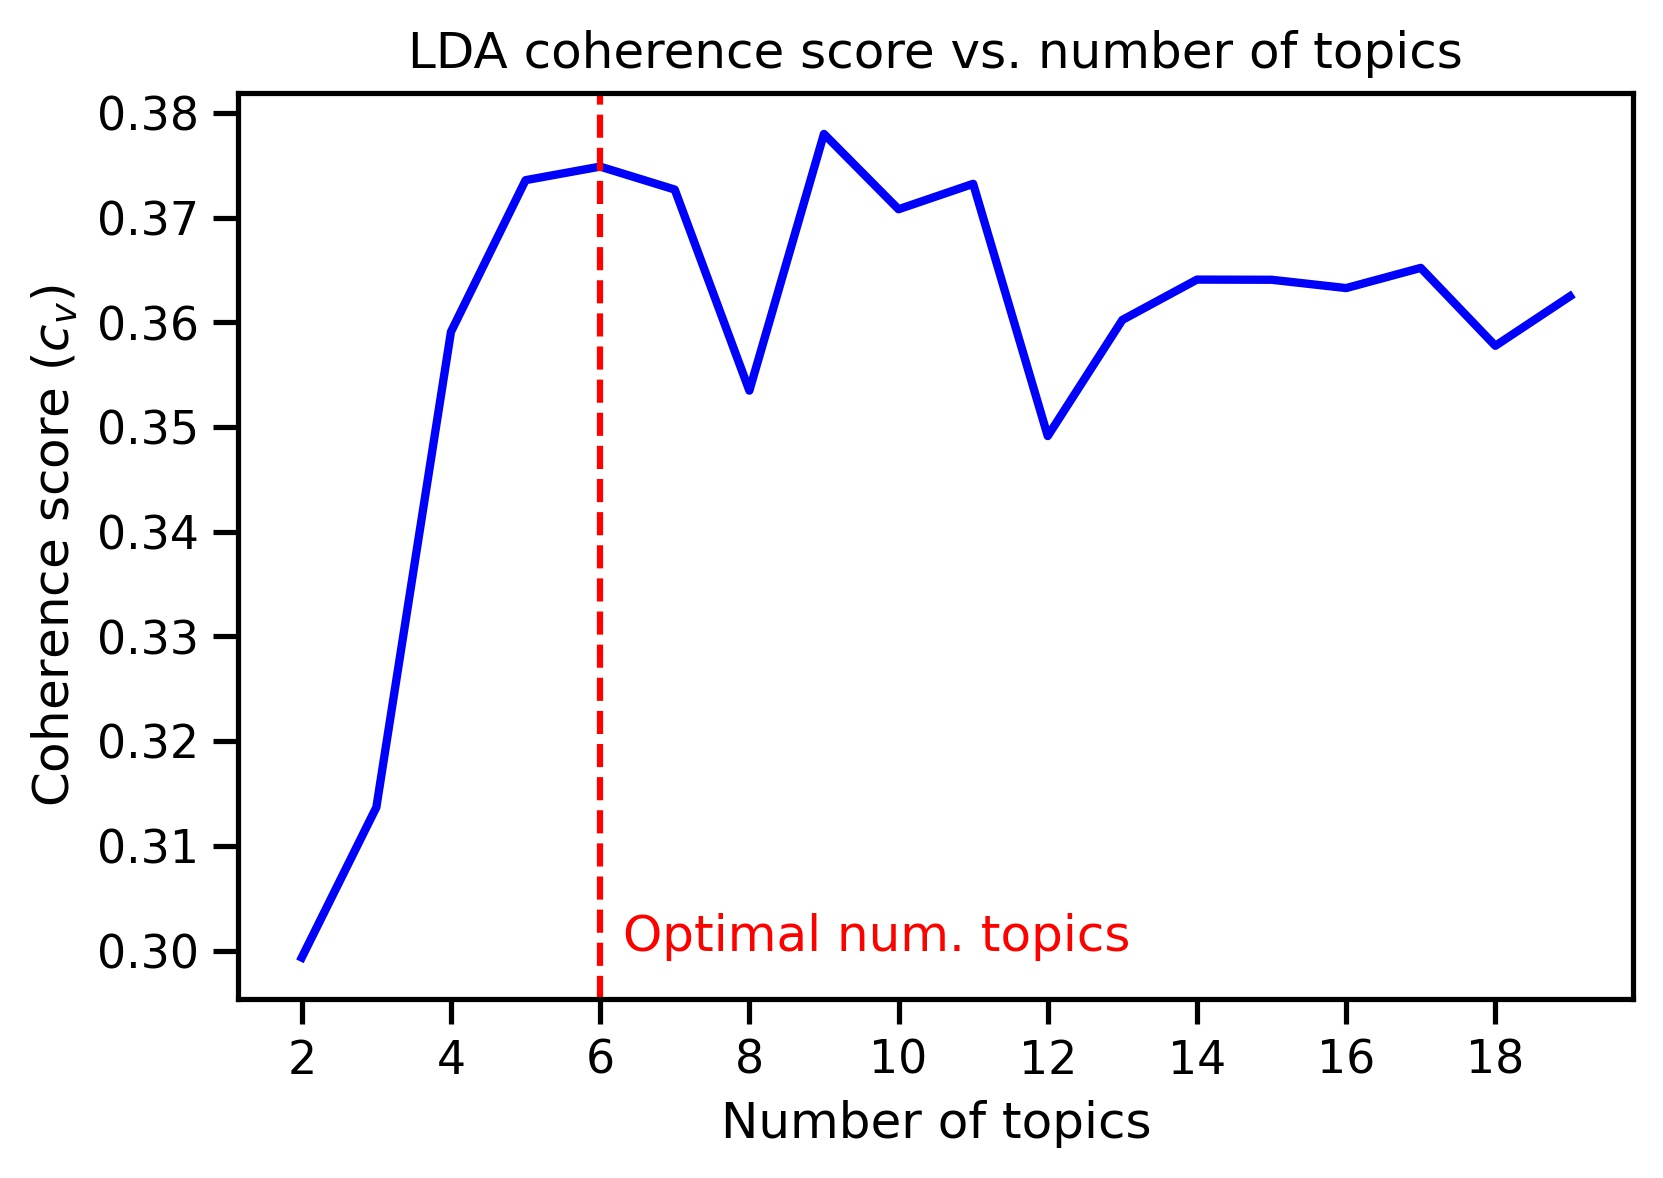
\includegraphics[scale = 0.5]{LDA_coherence}
				\end{center}
			\end{figure}
		\end{column}
		
		
	\end{columns}
Tuning from 2-20 topics: 6 looks good. 
\end{frame}
	\begin{frame}{Visualizing the topic model}
	
	\begin{figure}[H]
		\begin{center}
			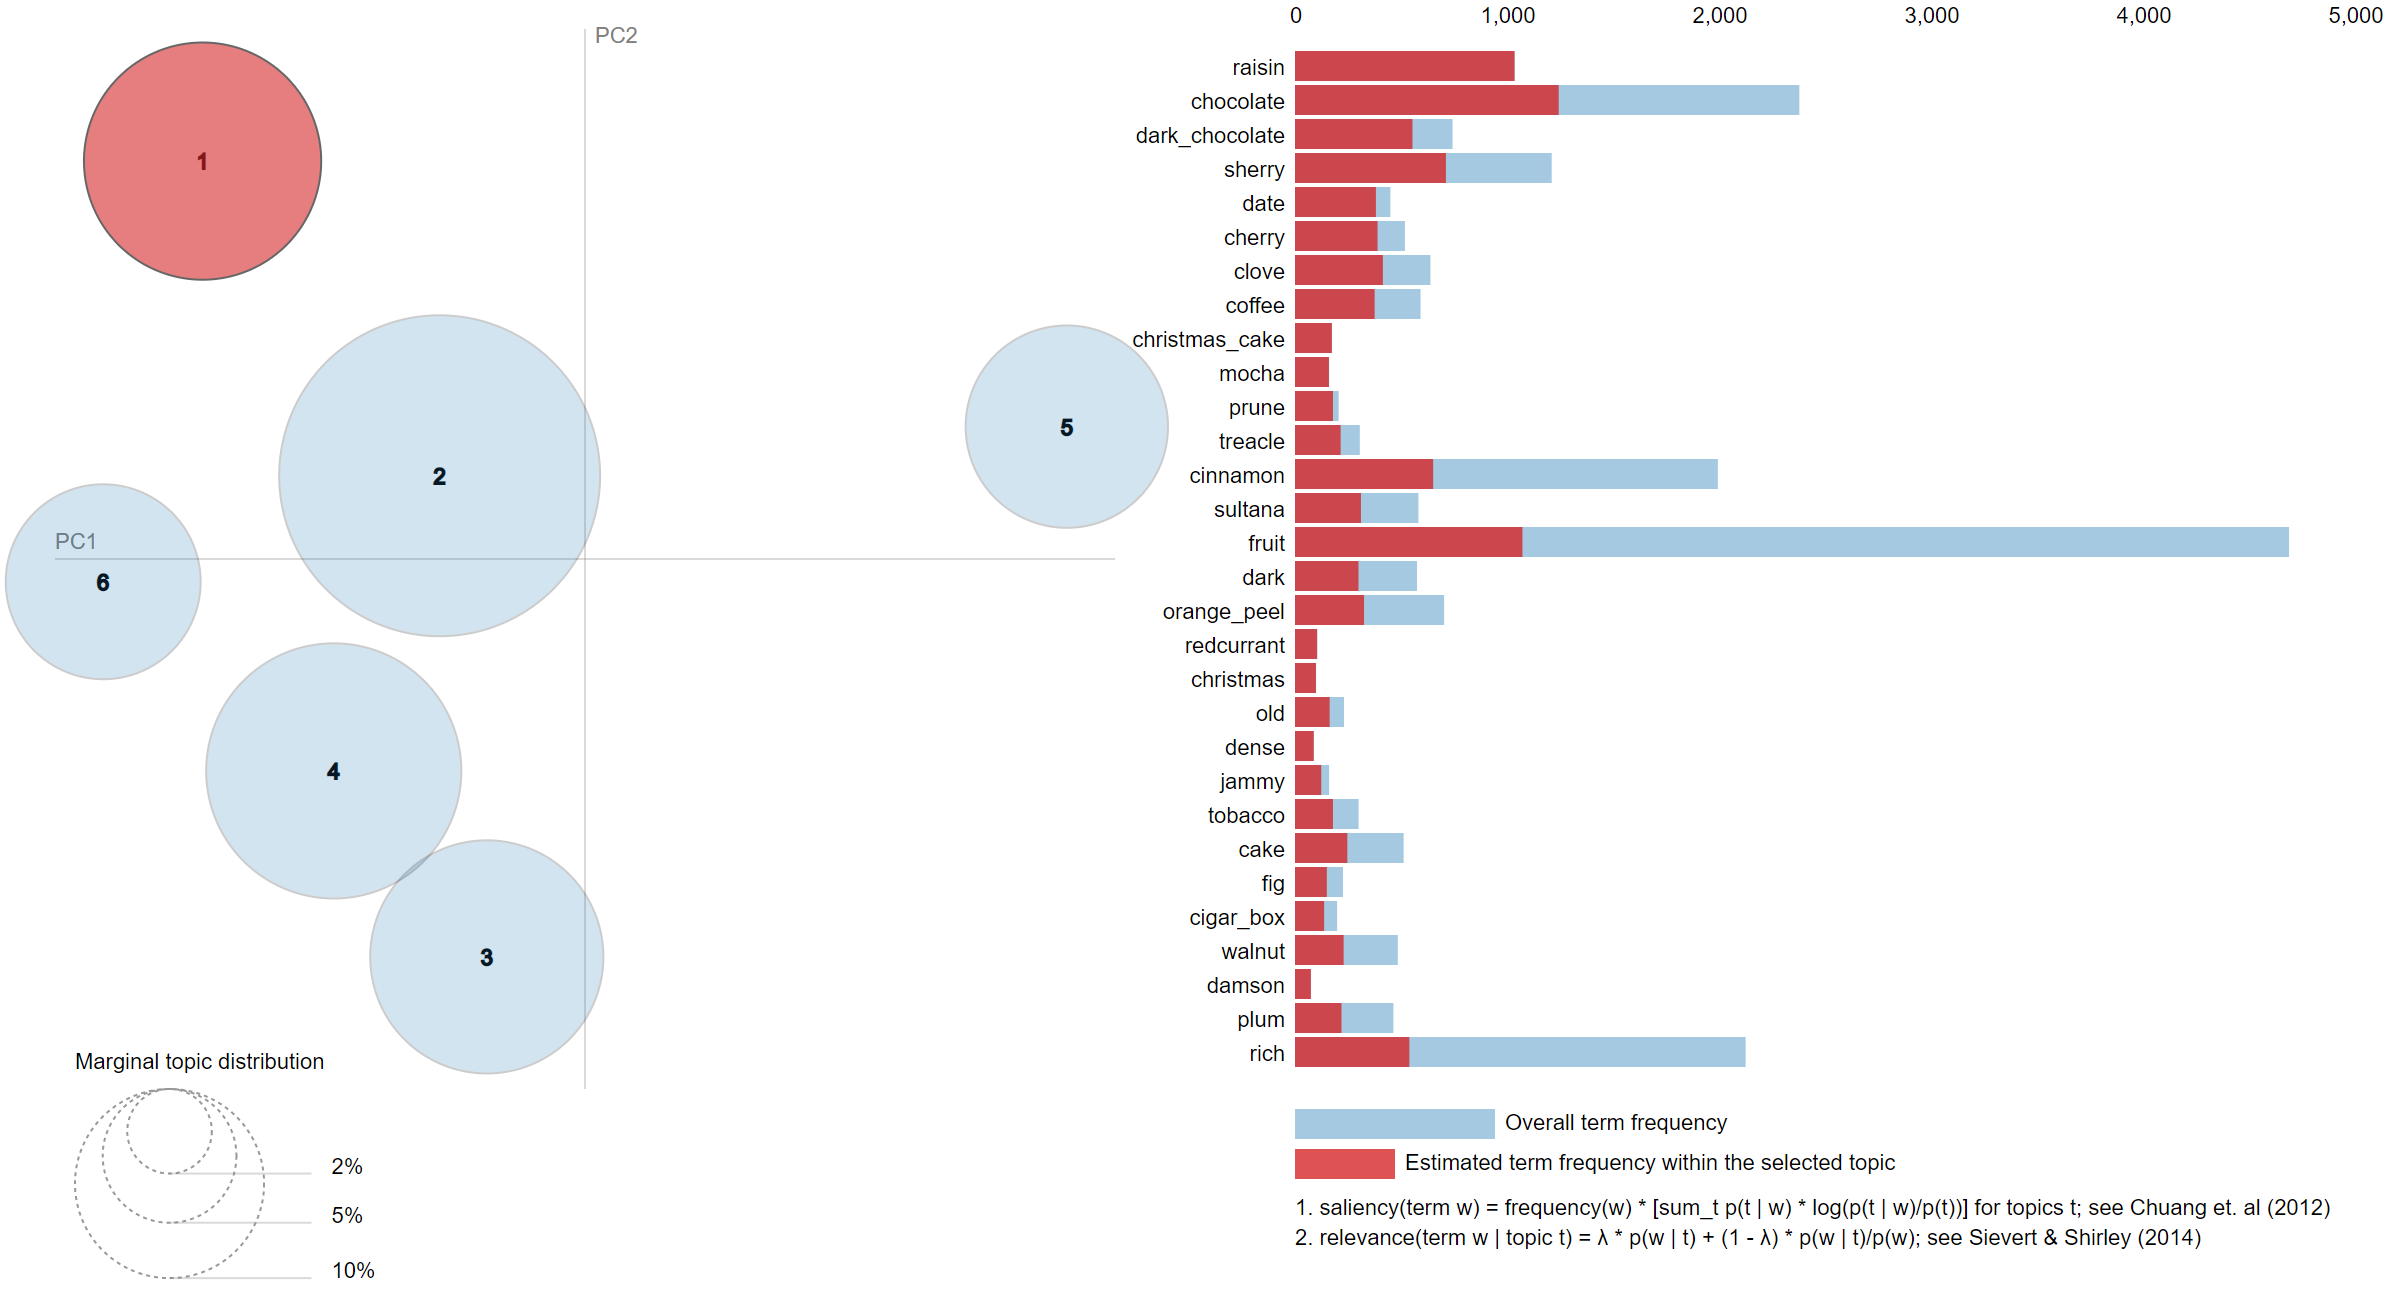
\includegraphics[scale = 0.37]{PyLDAvis_topmodel1}
		\end{center}
	\end{figure}
	
\end{frame}
\begin{frame}{Visualizing the topic model}
	
	\begin{figure}[H]
		\begin{center}
			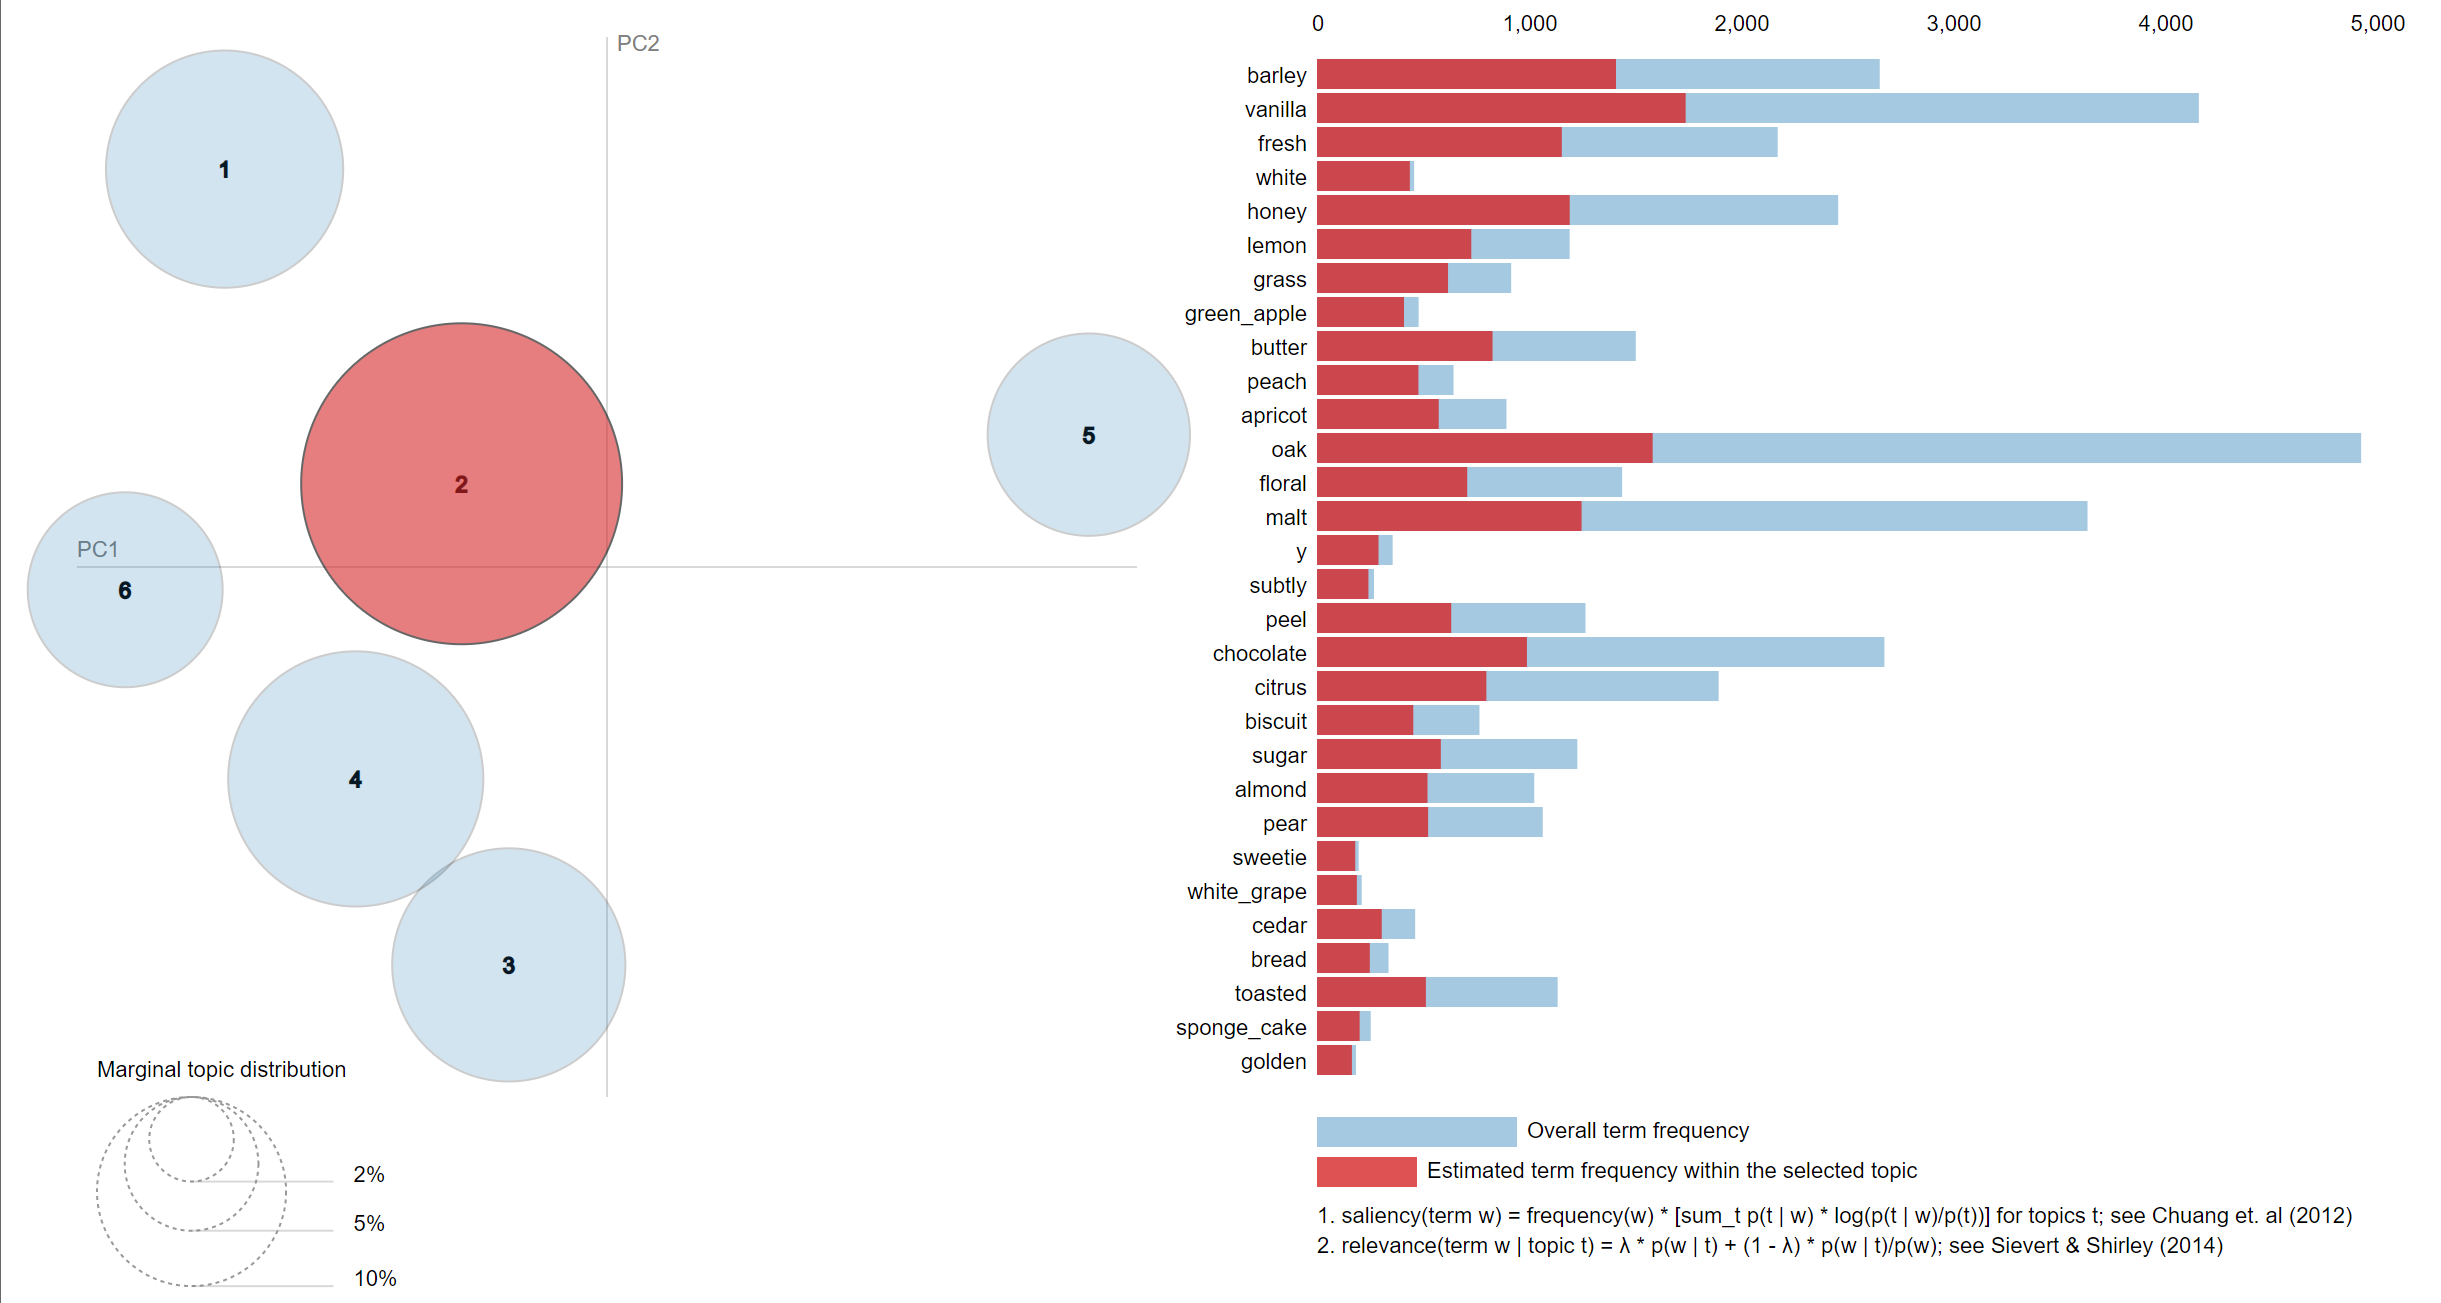
\includegraphics[scale = 0.37]{PyLDAvis_topmodel2}
		\end{center}
	\end{figure}
\end{frame}
	\begin{frame}{Visualizing the topic model}

			\begin{figure}[H]
				\begin{center}
					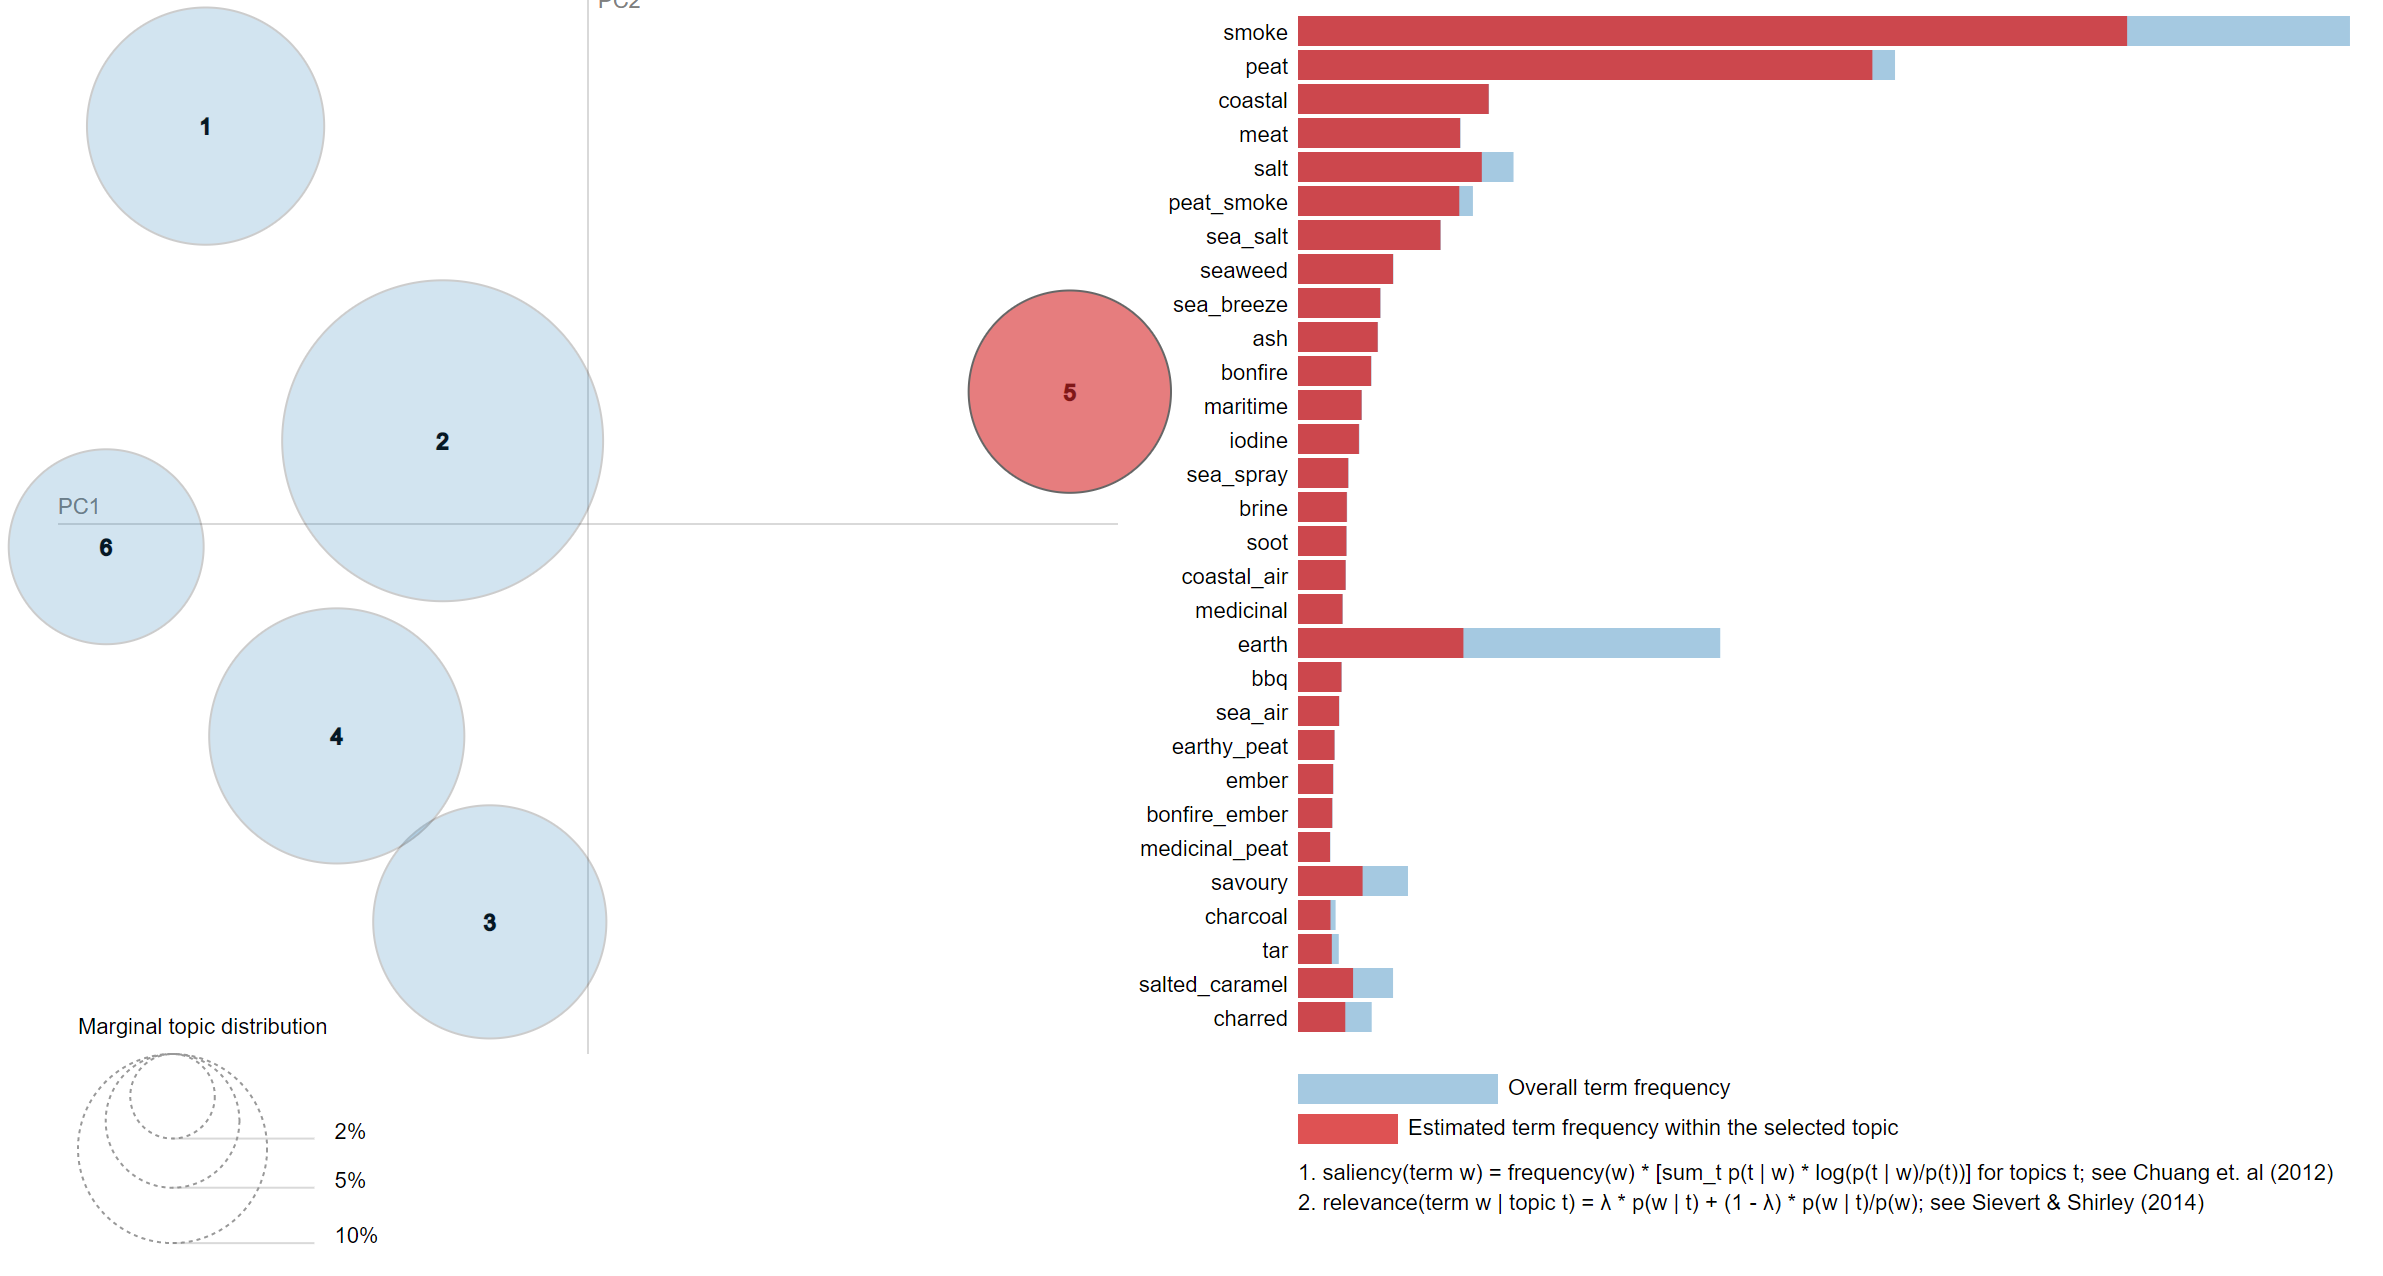
\includegraphics[scale = 0.37]{PyLDAvis_topmodel5}
				\end{center}
			\end{figure}

\end{frame}

	\begin{frame}{Gist of the topics}
		
		\begin{adjustbox}{max totalsize={.9\textwidth}{.7\textheight},center}
			
			\begin{tabular}{|c|c|}
				\hline
				\textbf{Topics} &  \textbf{Description}\\
				\hline
				1 & Aromatic spice, candied fruit, molasses, Christmas. Dark, sweet flavors. \\
				\hline
				2 & Citrus and floral with cream, malty notes. \\
				\hline
				3 & Herbal, tannin, citrus, wood spice. Drier notes. \\
				\hline
				4 & Wood, smoke, and pepper/heat. But also combined with cream and custard. Richness.  \\
				\hline
				5 & Smoke, peat, salt, meat. All the savoury notes. \\
				\hline
				6 & Berries, rhubarb, dark chocolate, jam, fruits, tartness but sweet.  \\
				\hline
			\end{tabular}
			
			
			
		\end{adjustbox}
\begin{columns}
	\begin{column}{0.5\textwidth}
		\begin{figure}
		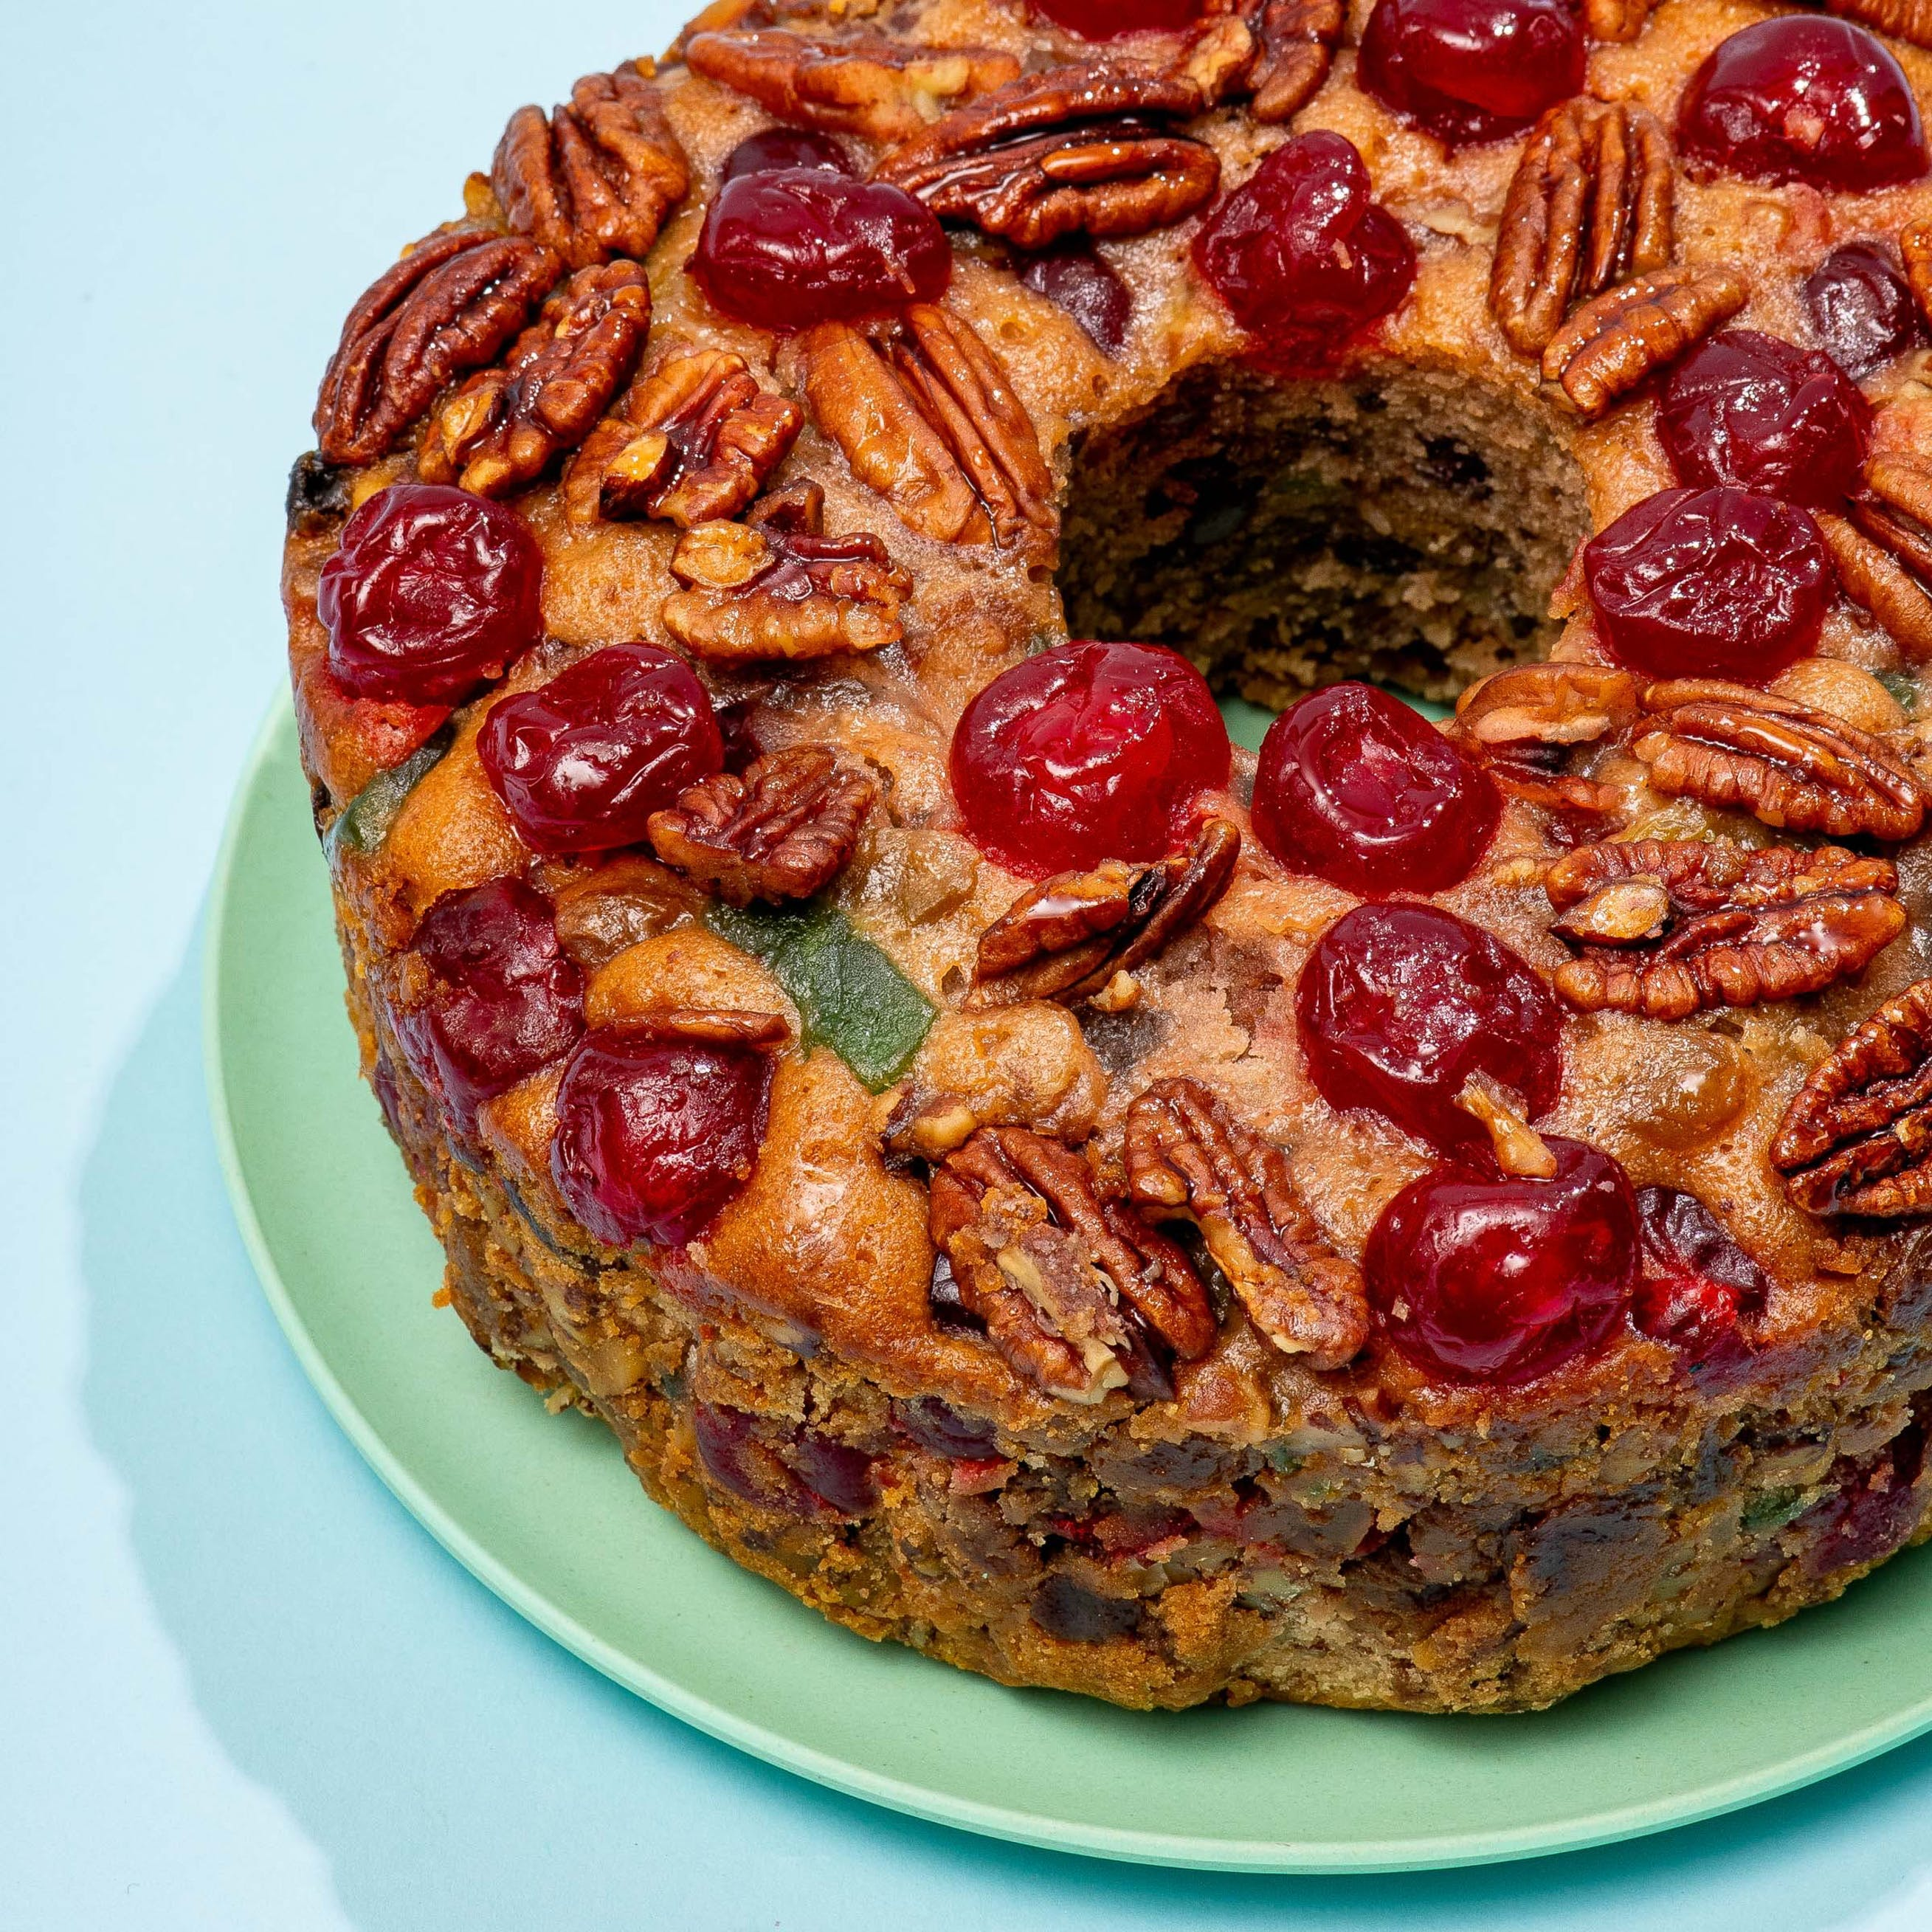
\includegraphics[scale = 0.04]{christmas_cake}
		\caption{Topic 1: Christmas cake}
		\end{figure}
		\end{column}
	\begin{column}{0.5\textwidth}
			\begin{figure}
		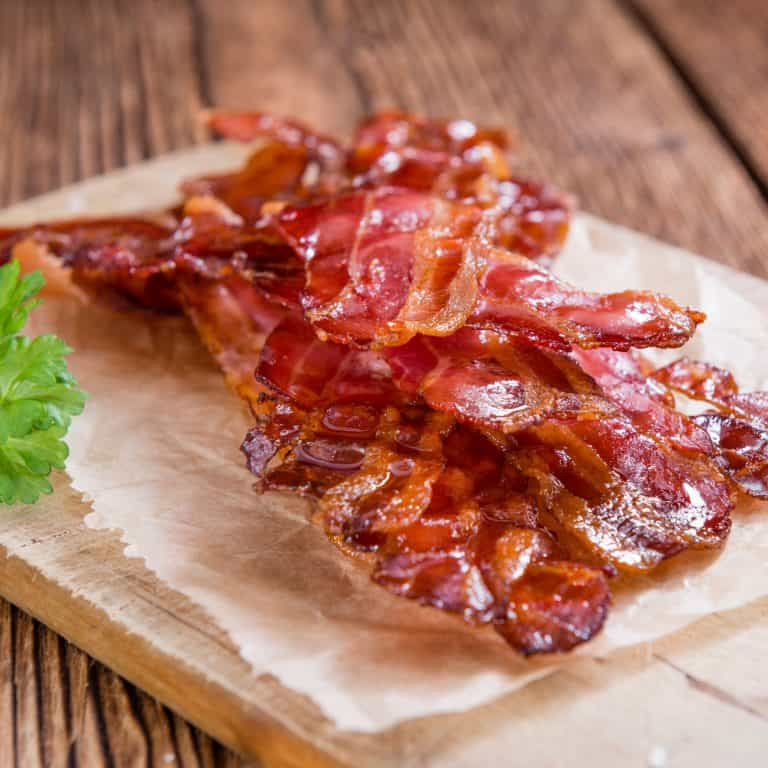
\includegraphics[scale = 0.14]{bacon}
		\caption{Topic 5: Bacon. }
	\end{figure}
	\end{column}
\end{columns}
	
	
\end{frame}

	\begin{frame}{Taste profile comparison: Islay Scotches}
		\fontsize{8pt}{8pt}\selectfont
		
			\begin{columns}
		\begin{column}{0.4\textwidth}
				\begin{itemize}
				\item \textbf{Ardbeg 10}: sweet, vanilla, lemon, lime, ardbeg, smoke, love, ridge, vanilla, mountain, peat, citrus, fruit, cloud, sea\_spray, long, glorious, sea, caramel, beach\_bonfire, smoke
				\item \textbf{Laphroaig 10}: 'seaweed', 'vanilla', 'ice\_cream','tcp', 'plaster', 'oak', 'spice', 'cardamom', 'black\_pepper', 'chilli', 'big', 'muscular', 'peat', 'spice', 'liquorice', 'big', 'dose', 'salt', 'slightly', 'sweet', 'beauty', 'classic', 'iodine', 'plaster', 'cool\_wood', 'smoke', 'big', 'savoury', 'tarry', 'iodine'
			\end{itemize}
		\end{column}
		\begin{column}{0.6\textwidth}
			\begin{figure}[H]
				\begin{center}
					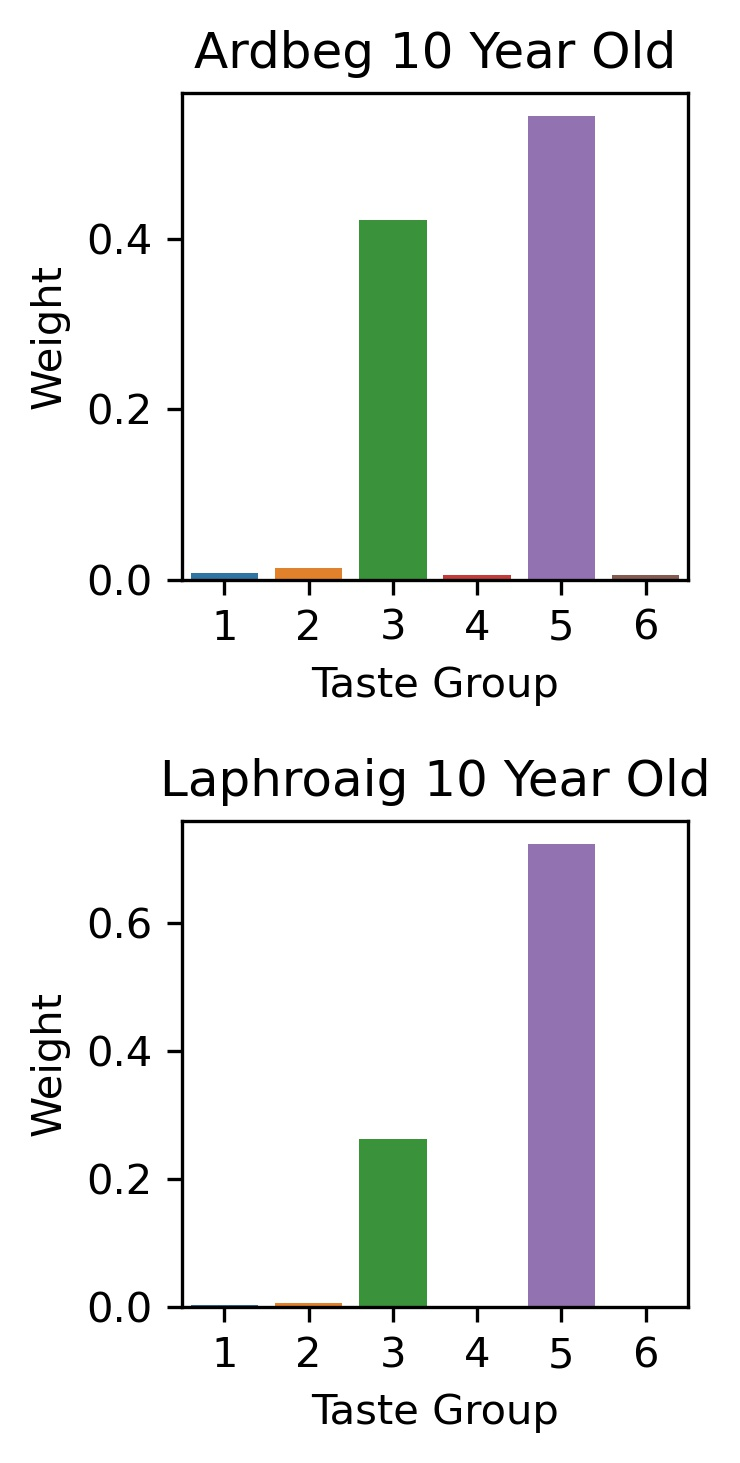
\includegraphics[scale = 0.5]{islaycomptopics}
					\caption{Taste group 3 = Herbal, tannin, citrus, wood spice. Drier notes. Taste group 5 = Peaty, salty, meaty notes.}
			\end{center}
			\end{figure}
		\end{column}
		
		
	\end{columns}
\end{frame}
	\begin{frame}{Taste profile comparison: Effect of Sherry Finish}
	\fontsize{8pt}{8pt}\selectfont
	
	\begin{columns}
		\begin{column}{0.4\textwidth}
			\begin{itemize}
				\item \textbf{Laphroaig 10}: 'seaweed', 'vanilla', 'ice\_cream','tcp', 'plaster', 'oak', 'spice', 'cardamom', 'black\_pepper', 'chilli', 'big', 'muscular', 'peat', 'spice', 'liquorice', 'big', 'dose', 'salt', 'slightly', 'sweet', 'beauty', 'classic', 'iodine', 'plaster', 'cool\_wood', 'smoke', 'big', 'savoury', 'tarry', 'iodine'
				
				\item \textbf{Laphroaig 10 Sherry Finish}: 'roasted', 'cedar', 'peat\_smoke', 'iodine', 'away', 'dark\_chocolate', 'honey', 'vanilla\_pod', 'meat', 'maple\_syrup', 'bbq', 'lemon', 'charred\_oak', 'smidge', 'coffee', 'balanced', 'finish', 'sherry', 'sweet', 'smouldering', 'peat'
			\end{itemize}
		\end{column}
		\begin{column}{0.6\textwidth}
			\begin{figure}[H]
				\begin{center}
					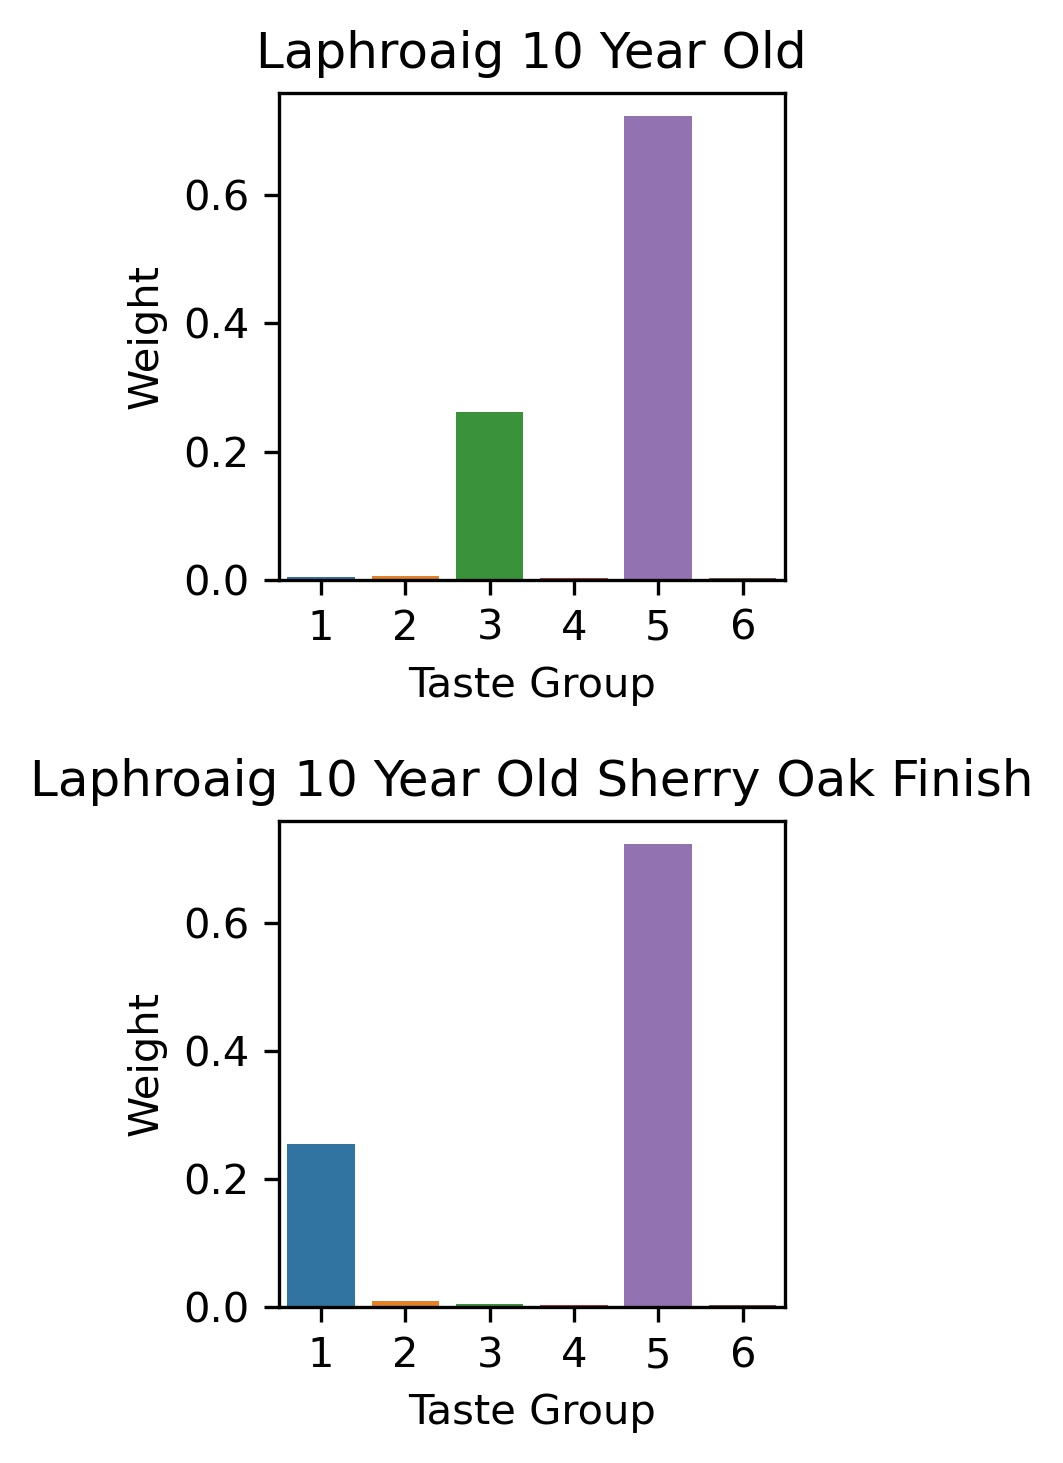
\includegraphics[scale = 0.5]{islaysherrying_comptopics}
					\caption{Taste group 3 = Herbal, tannin, citrus, wood spice. Drier notes. Taste group 5 = Peaty, salty, meaty notes. Taste group 1 = Nuts, molasses, candied berries, aromatic spice, and dark chocolate. Dark, sweet flavors}
				\end{center}
			\end{figure}
		\end{column}
		
		
	\end{columns}
\end{frame}

	\begin{frame}{Taste profile comparison: On the sweeter side}
	\fontsize{8pt}{8pt}\selectfont
	
	\begin{columns}
		\begin{column}{0.4\textwidth}
			\begin{itemize}
				\item \textbf{Aberlour A'Bunadh}: 'gingerbread', 'orange\_zest', 'black\_pepper', 'thick', 'sherry', 'vanilla\_pod', 'christmas\_cake', 'cherry', 'bakewells', 'hefty', 'helping', 'cinnamon', 'cedar', 'cinnamon', 'raisin'
				
				\item \textbf{Glenmorangie Nectar d'Or}: 'silk', 'syrup', 'syrup', 'sponge', 'vanilla', 'custard', 'butter', 'baklava', 'toasted', 'brown\_sugar', 'sweet', 'citrus', 'lemon\_curd', 'vanilla', 'shortbread', 'oak', 'spice', 'gingerbread', 'fruit', 'drizzle', 'runny\_honey', 'dry', 'oak', 'lemon', 'shortbread', 'gingersnap\_biscuit'
			\end{itemize}
		\end{column}
		\begin{column}{0.6\textwidth}
			\begin{figure}[H]
				\begin{center}
					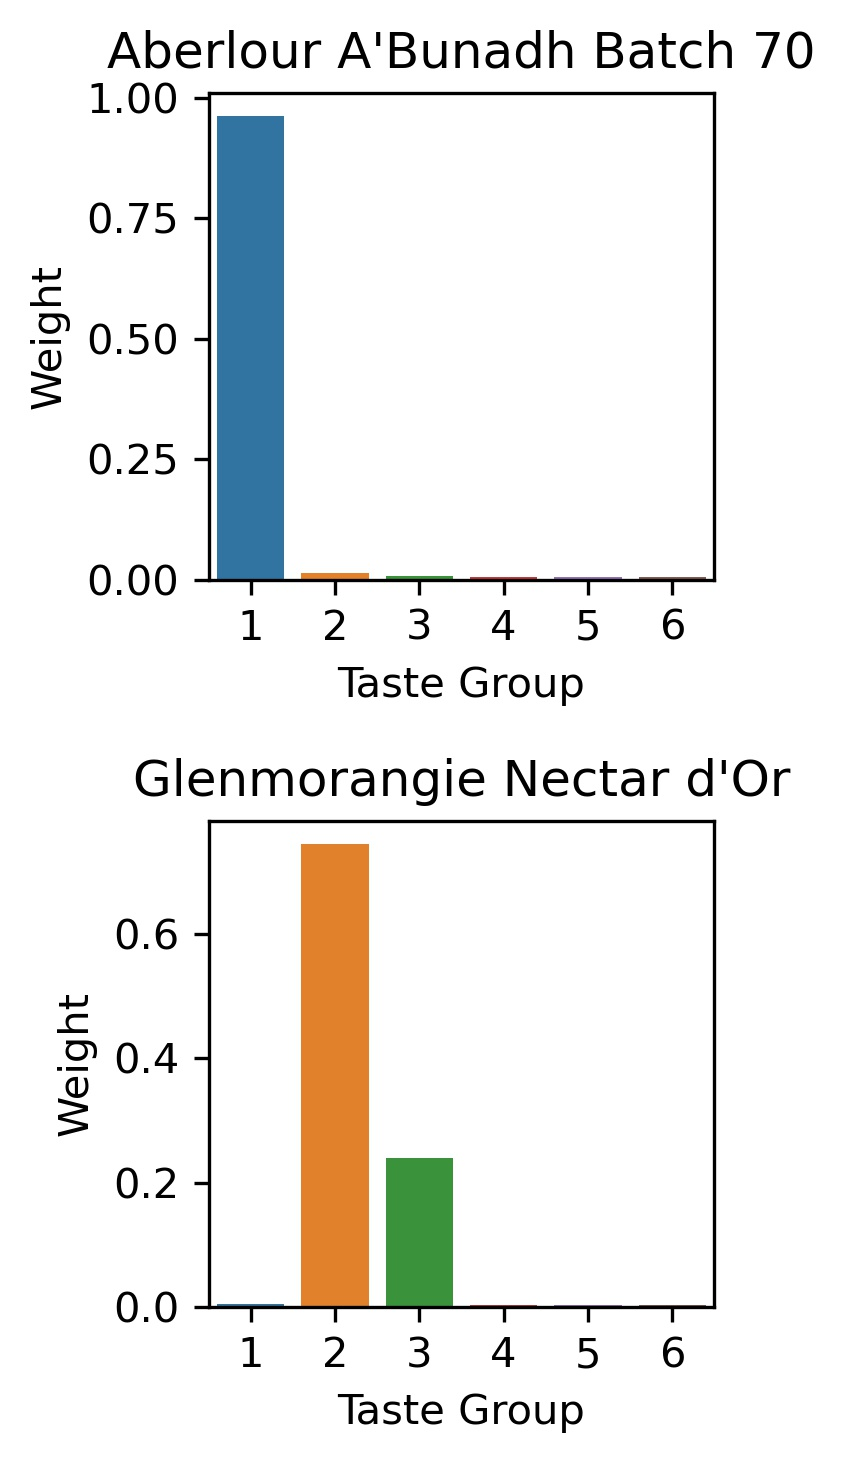
\includegraphics[scale = 0.5]{sweetsidetopics}
					\caption{ Taste group 1 = Nuts, molasses, candied berries, aromatic spice, and dark chocolate. Dark, sweet flavors. Taste group 2 = Citrus and floral with cream, malty notes. Taste group 3 = Herbal, tannin, citrus, wood spice. Drier notes.}
				\end{center}
			\end{figure}
		\end{column}
		
		
	\end{columns}
\end{frame}
\begin{frame}{Building Recommendation Engine}
	\begin{itemize}
		\item Scotch review as topic vector
		\item Cosine similarity and ranking
	\end{itemize}
\begin{figure}[H]

		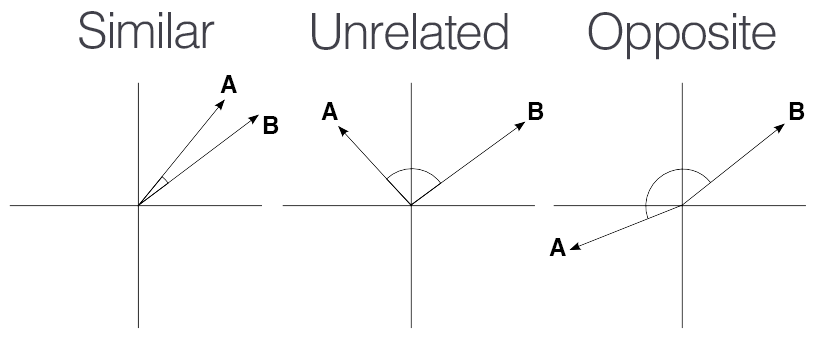
\includegraphics[scale = 0.175]{sim_metric_cosine}

\end{figure}
\textbf{In-Corpus}: rank similarity of scotches to input scotch (all in corpus). Gensim index similarities. \\
\textbf{Out-of-Corpus}: Free text input of tastes. Get scotch recommendations.
	\begin{block}{Out-of-corpus recommender flow}
	\begin{adjustbox}{max totalsize={.9\textwidth}{.7\textheight},center}
		
		\begin{tikzpicture}[>=latex']
			
			\node [block] (start) {Free text input};
			\node [block, right =0.5cm of start] (preprocess) {Processing \\ + \\ tokenization  };
			\node [block, right =0.5cm of preprocess] (statdetector) {BoW \\ from \\ dictionary};
			\node [block, right =0.5cm of statdetector] (otsu) {Topic breakdown};
			\node [block, right =0.5cm of otsu] (rec) {Cosine sim. with corpus};
			
			
			%% paths
			\path[draw,->]
			(start) edge (preprocess)
			(preprocess) edge (statdetector)
			(statdetector) edge (otsu)
			(otsu) edge (rec)
			;
		\end{tikzpicture}
		
	\end{adjustbox}
\end{block}
\end{frame}
	
\begin{frame}{In-corpus recommendations}
	\textbf{Aberlour A'Bunadh}: 'gingerbread', 'orange\_zest', 'black\_pepper', 'thick', 'sherry', 'vanilla\_pod', 'christmas\_cake', 'cherry', 'bakewells', 'hefty', 'helping', 'cinnamon', 'cedar', 'cinnamon', 'raisin'
	\begin{columns}
		\begin{column}{0.5\textwidth}
			
			'brown\_sugar', 'treacle', 'clove', 'cinnamon', 'load', 'raisin', 'walnut\_loaf', 'damson\_jam', 'richly', 'chocolate', 'rum', 'like', 'spice', 'chocolate', 'date'
 
		\end{column}
		\begin{column}{0.5\textwidth}
			\begin{figure}
			\begin{center}
				Edradour 10 Year Old
				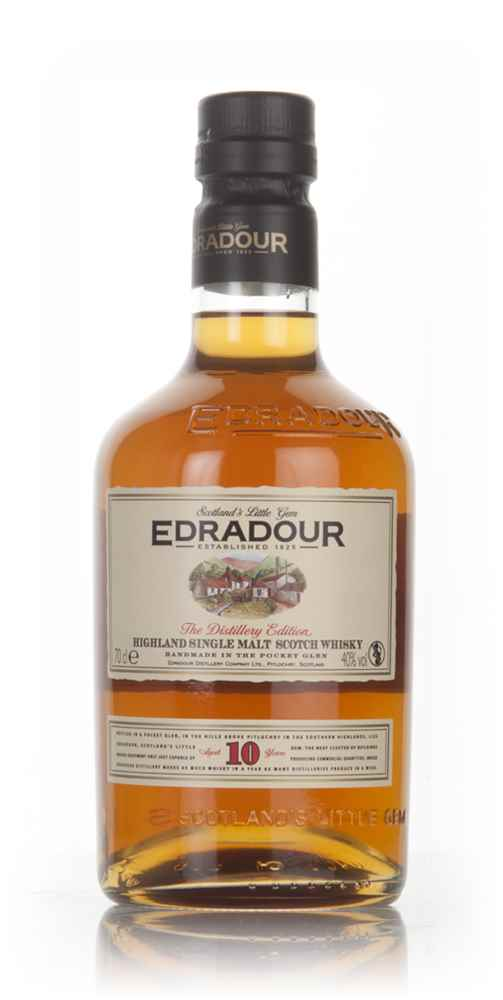
\includegraphics[scale = 0.2]{edradour10}
			\end{center}
		\end{figure}
		\end{column}
	\end{columns}


	
\end{frame}

\begin{frame}{In-corpus recommendations}
	\textbf{Aberlour A'Bunadh}: 'gingerbread', 'orange\_zest', 'black\_pepper', 'thick', 'sherry', 'vanilla\_pod', 'christmas\_cake', 'cherry', 'bakewells', 'hefty', 'helping', 'cinnamon', 'cedar', 'cinnamon', 'raisin'
	\begin{columns}
		\begin{column}{0.5\textwidth}
			
			'soft', 'red', 'fruit', 'brown\_sugar', 'clove', 'chocolate', 'brazil\_nut', 'dry', 'orange\_peel', 'red\_wine', 'pecan', 'raspberry\_jam', 'crystallised\_ginger', 'cacao', 'juicy', 'blackcurrant'
			
		\end{column}
		\begin{column}{0.5\textwidth}
			\begin{figure}
				\begin{center}
					Tamdhu 10 Year Old
					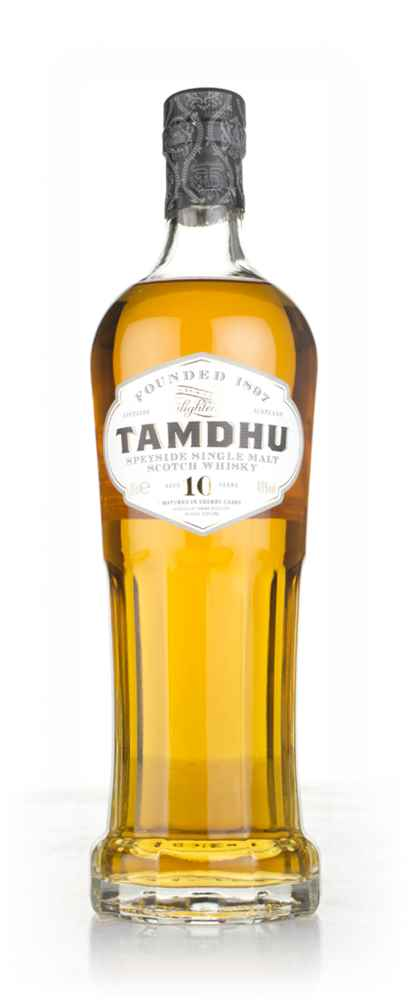
\includegraphics[scale = 0.2]{tamdhu10}
				\end{center}
			\end{figure}
		\end{column}
	\end{columns}
	
	
	
\end{frame}

	\begin{frame}{Out-of-corpus recommendation}
		\textbf{Text input}: "light, citrus, lemon, grapefruit, dry, crisp, sea salt, salted caramel"
	
		\begin{columns}
			\begin{column}{0.5\textwidth}
				\textbf{Recommendation:}
				\textit{Tasting Notes}: 'light', 'sweet', 'green', 'grape', 'rhubarb', 'great', 'contrast', 'big', 'blast', 'smoke', 'salt', 'leather', 'maritime', 'combination', 'harbourmaster', 'jacket', 'salt'.
			\end{column}
					\begin{column}{0.5\textwidth}
						\begin{figure}[H]
						\begin{center}
							Longrow Peated
						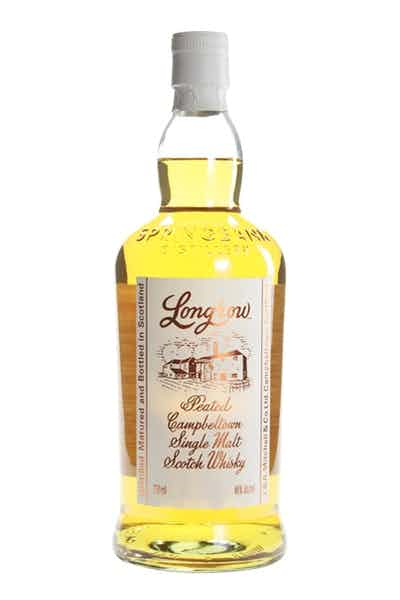
\includegraphics[scale = 0.3]{longrow_peated}
						\end{center}
					\end{figure}
		\end{column}
		\end{columns}	
\end{frame}


\begin{frame}{Conclusion/Future Directions}
\begin{itemize}
	\item Dictionary for Scotch tasting notes
	\item Different meaningful sectors of taste descriptors
	\item LDA Topic model captures general taste profiles of Scotches
	\item Room for improvement:
	\begin{itemize}
		\item Topics (vector) orthogonal but topics actually have some overlap (Topics 1 and 6, 3 and 4)
		\item When is a taste descriptor 'big' ? Or when is it just a 'hint of' a given descriptor? Degree.
		\item LDA + word embedding model for context?
	\end{itemize}
\item Get me some of that Longrow Peated and have a whee dram by the fireplace this evening!
\end{itemize}

\end{frame}
\end{document}